% Options for packages loaded elsewhere
\PassOptionsToPackage{unicode}{hyperref}
\PassOptionsToPackage{hyphens}{url}
\PassOptionsToPackage{dvipsnames,svgnames,x11names}{xcolor}
%
\documentclass[
  letterpaper,
  DIV=11,
  numbers=noendperiod]{scrartcl}

\usepackage{amsmath,amssymb}
\usepackage{iftex}
\ifPDFTeX
  \usepackage[T1]{fontenc}
  \usepackage[utf8]{inputenc}
  \usepackage{textcomp} % provide euro and other symbols
\else % if luatex or xetex
  \usepackage{unicode-math}
  \defaultfontfeatures{Scale=MatchLowercase}
  \defaultfontfeatures[\rmfamily]{Ligatures=TeX,Scale=1}
\fi
\usepackage{lmodern}
\ifPDFTeX\else  
    % xetex/luatex font selection
\fi
% Use upquote if available, for straight quotes in verbatim environments
\IfFileExists{upquote.sty}{\usepackage{upquote}}{}
\IfFileExists{microtype.sty}{% use microtype if available
  \usepackage[]{microtype}
  \UseMicrotypeSet[protrusion]{basicmath} % disable protrusion for tt fonts
}{}
\makeatletter
\@ifundefined{KOMAClassName}{% if non-KOMA class
  \IfFileExists{parskip.sty}{%
    \usepackage{parskip}
  }{% else
    \setlength{\parindent}{0pt}
    \setlength{\parskip}{6pt plus 2pt minus 1pt}}
}{% if KOMA class
  \KOMAoptions{parskip=half}}
\makeatother
\usepackage{xcolor}
\setlength{\emergencystretch}{3em} % prevent overfull lines
\setcounter{secnumdepth}{-\maxdimen} % remove section numbering
% Make \paragraph and \subparagraph free-standing
\makeatletter
\ifx\paragraph\undefined\else
  \let\oldparagraph\paragraph
  \renewcommand{\paragraph}{
    \@ifstar
      \xxxParagraphStar
      \xxxParagraphNoStar
  }
  \newcommand{\xxxParagraphStar}[1]{\oldparagraph*{#1}\mbox{}}
  \newcommand{\xxxParagraphNoStar}[1]{\oldparagraph{#1}\mbox{}}
\fi
\ifx\subparagraph\undefined\else
  \let\oldsubparagraph\subparagraph
  \renewcommand{\subparagraph}{
    \@ifstar
      \xxxSubParagraphStar
      \xxxSubParagraphNoStar
  }
  \newcommand{\xxxSubParagraphStar}[1]{\oldsubparagraph*{#1}\mbox{}}
  \newcommand{\xxxSubParagraphNoStar}[1]{\oldsubparagraph{#1}\mbox{}}
\fi
\makeatother


\providecommand{\tightlist}{%
  \setlength{\itemsep}{0pt}\setlength{\parskip}{0pt}}\usepackage{longtable,booktabs,array}
\usepackage{calc} % for calculating minipage widths
% Correct order of tables after \paragraph or \subparagraph
\usepackage{etoolbox}
\makeatletter
\patchcmd\longtable{\par}{\if@noskipsec\mbox{}\fi\par}{}{}
\makeatother
% Allow footnotes in longtable head/foot
\IfFileExists{footnotehyper.sty}{\usepackage{footnotehyper}}{\usepackage{footnote}}
\makesavenoteenv{longtable}
\usepackage{graphicx}
\makeatletter
\def\maxwidth{\ifdim\Gin@nat@width>\linewidth\linewidth\else\Gin@nat@width\fi}
\def\maxheight{\ifdim\Gin@nat@height>\textheight\textheight\else\Gin@nat@height\fi}
\makeatother
% Scale images if necessary, so that they will not overflow the page
% margins by default, and it is still possible to overwrite the defaults
% using explicit options in \includegraphics[width, height, ...]{}
\setkeys{Gin}{width=\maxwidth,height=\maxheight,keepaspectratio}
% Set default figure placement to htbp
\makeatletter
\def\fps@figure{htbp}
\makeatother

\KOMAoption{captions}{tableheading}
\makeatletter
\@ifpackageloaded{caption}{}{\usepackage{caption}}
\AtBeginDocument{%
\ifdefined\contentsname
  \renewcommand*\contentsname{Table of contents}
\else
  \newcommand\contentsname{Table of contents}
\fi
\ifdefined\listfigurename
  \renewcommand*\listfigurename{List of Figures}
\else
  \newcommand\listfigurename{List of Figures}
\fi
\ifdefined\listtablename
  \renewcommand*\listtablename{List of Tables}
\else
  \newcommand\listtablename{List of Tables}
\fi
\ifdefined\figurename
  \renewcommand*\figurename{Figure}
\else
  \newcommand\figurename{Figure}
\fi
\ifdefined\tablename
  \renewcommand*\tablename{Table}
\else
  \newcommand\tablename{Table}
\fi
}
\@ifpackageloaded{float}{}{\usepackage{float}}
\floatstyle{ruled}
\@ifundefined{c@chapter}{\newfloat{codelisting}{h}{lop}}{\newfloat{codelisting}{h}{lop}[chapter]}
\floatname{codelisting}{Listing}
\newcommand*\listoflistings{\listof{codelisting}{List of Listings}}
\makeatother
\makeatletter
\makeatother
\makeatletter
\@ifpackageloaded{caption}{}{\usepackage{caption}}
\@ifpackageloaded{subcaption}{}{\usepackage{subcaption}}
\makeatother

\ifLuaTeX
  \usepackage{selnolig}  % disable illegal ligatures
\fi
\usepackage{bookmark}

\IfFileExists{xurl.sty}{\usepackage{xurl}}{} % add URL line breaks if available
\urlstyle{same} % disable monospaced font for URLs
\hypersetup{
  pdftitle={Christmas 2004},
  colorlinks=true,
  linkcolor={blue},
  filecolor={Maroon},
  citecolor={Blue},
  urlcolor={Blue},
  pdfcreator={LaTeX via pandoc}}


\title{Christmas 2004}
\author{}
\date{}

\begin{document}
\maketitle


\subsection{Cast}\label{cast}

\begin{itemize}
\tightlist
\item
  Mary a young women who is about to deliver a baby
\item
  Joseph - Her husband - faithful but a bit puzzled
\item
  Innkeeper - Small business owner in Bethleham
\item
  Chief Sheep - Extroverted leader sheep
\item
  Under-sheep - Extroverted junior sheep (not used to following the
  crowd
\item
  Angels - God's ``shock and awe'' messengers
\end{itemize}

\subsection{}\label{section}

She was very happy

She was a virgin Promised to be married

Mary and Joseph had to take a trip

They looked for a place to sleep as she was expecting a child

Finally, the inkeeper said that they could at

Many people, but no room for them at the inn

Stable with animals

Joseph made a soft bed for Mary

God's son was born that night

\textbf{Mary wrapped him in soft cloths and laid him in a manger. She
named her baby Jesus}

\subsection{Away in an Manger}\label{away-in-an-manger}

Away in a manger, no crib for a bed

The little Lord Jesus laid down His sweet head

The stars in the bright sky looked down where He lay

The little Lord Jesus asleep on the hay

\subsection{}\label{section-1}

\textbf{A savior is born in Bethleham. You will find him wrapped in
swaddling clothes and lying in a manger}

\subsection{First Noel (1)}\label{first-noel-1}

The first Noel the angel did say

was to certain poor shepherds in fields as they lay;

In fields where they lay tending their sheep,

On a cold win­ter's night that was so deep.\\
\strut \\
Noel, Noel, Noel, Noel.

Born is the King of Israel

\subsection{}\label{section-2}

``Let's see if we can find this baby''

They told everyone what

Suddenly thousands of angels appeared in the sky

Peace, Goodwill toward manking

\textbf{They praise God for sending Jesus to be our savior, saying
``Glory to God in the highest. And on earth peace, goodwill toward
men.''}

\subsection{Hark the Herald Angels
Sing}\label{hark-the-herald-angels-sing}

\begin{enumerate}
\def\labelenumi{\arabic{enumi}.}
\setcounter{enumi}{3}
\tightlist
\item
  They told everyone the good news. They praised God all the way back to
  their fields.
\end{enumerate}

\subsection{O Come All ye Faithful (1)}\label{o-come-all-ye-faithful-1}

O come, all ye faithful, joyful and triumphant

O come ye, o come ye to Bethlehem

O come and behold Him, born the King of Angels

O come, let us adore Him x3

Christ the Lord

O come, all ye faithful O come, all ye faithful O come, all ye faithful
to Bethlehem

O come, all ye faithful O come, all ye faithful O come, all ye faithful
to Bethlehem

\subsection{}\label{section-3}

\begin{quote}
When Jesus was about 2 years old
\end{quote}

\begin{quote}
Wise men gave gifts to Jesus and worshiped him. They knew he was to be a
great king.
\end{quote}

\subsection{We Three Kings of Orient
Are}\label{we-three-kings-of-orient-are}

\subsection{God Rest Ye Merry
Gentlemen}\label{god-rest-ye-merry-gentlemen}

God rest ye merry gentlemen Let nothing you dismay Remember Christ our
Savior Was born on Christmas Day To save us all from Satan's pow'r When
we were gone astray Oh tidings of comfort and joy Comfort and joy Oh
tidings of comfort and joy God rest ye merry gentlemen Let nothing you
dismay Remember Christ our Savior Was born on Christmas Day To save us
all from Satan's pow'r When we were gone astray Oh tidings of comfort
and joy Comfort and joy Oh tidings of comfort and joy In Bethlehem, in
Israel This blessed Babe was born And laid within a manger Upon this
blessed morn The which His Mother Mary Did nothing take in scorn Oh
tidings of comfort and joy Comfort and joy Oh tidings of comfort and joy
Fear not then, said the Angel Let nothing you affright This day is born
a Savior Of a pure Virgin bright To free all those who trust in Him From
Satan's pow'r and might Oh tidings of comfort and joy Comfort and joy Oh
tidings of comfort and joy God rest ye merry gentlemen Let nothing you
dismay Remember Christ our Savior Was born on Christmas Day To save us
all from Satan's pow'r When we were gone astray Oh tidings of comfort
and joy Comfort and joy Oh tidings of comfort and joy

\begin{center}\rule{0.5\linewidth}{0.5pt}\end{center}

\subsection{Hark the Herald A}\label{hark-the-herald-a}

\subsection{Silent Night (1)}\label{silent-night-1}

Silent night, holy night

All is calm, all is bright

Round yon Virgin, Mother and Child

Holy Infant so tender and mild

Sleep in heavenly peace

Sleep in heavenly peace

Silent night, holy night

Shepherds quake at the sight

Glories stream from heaven afar

Heavenly hosts sing Alleluia

Christ the Savior is born

Christ the Savior is born

\subsection{Anatomy}\label{anatomy}

Food moves from the throat

\(\rightarrow\) esophagus

\(\rightarrow\) stomach

\(\rightarrow\) small bowel (jejunum)

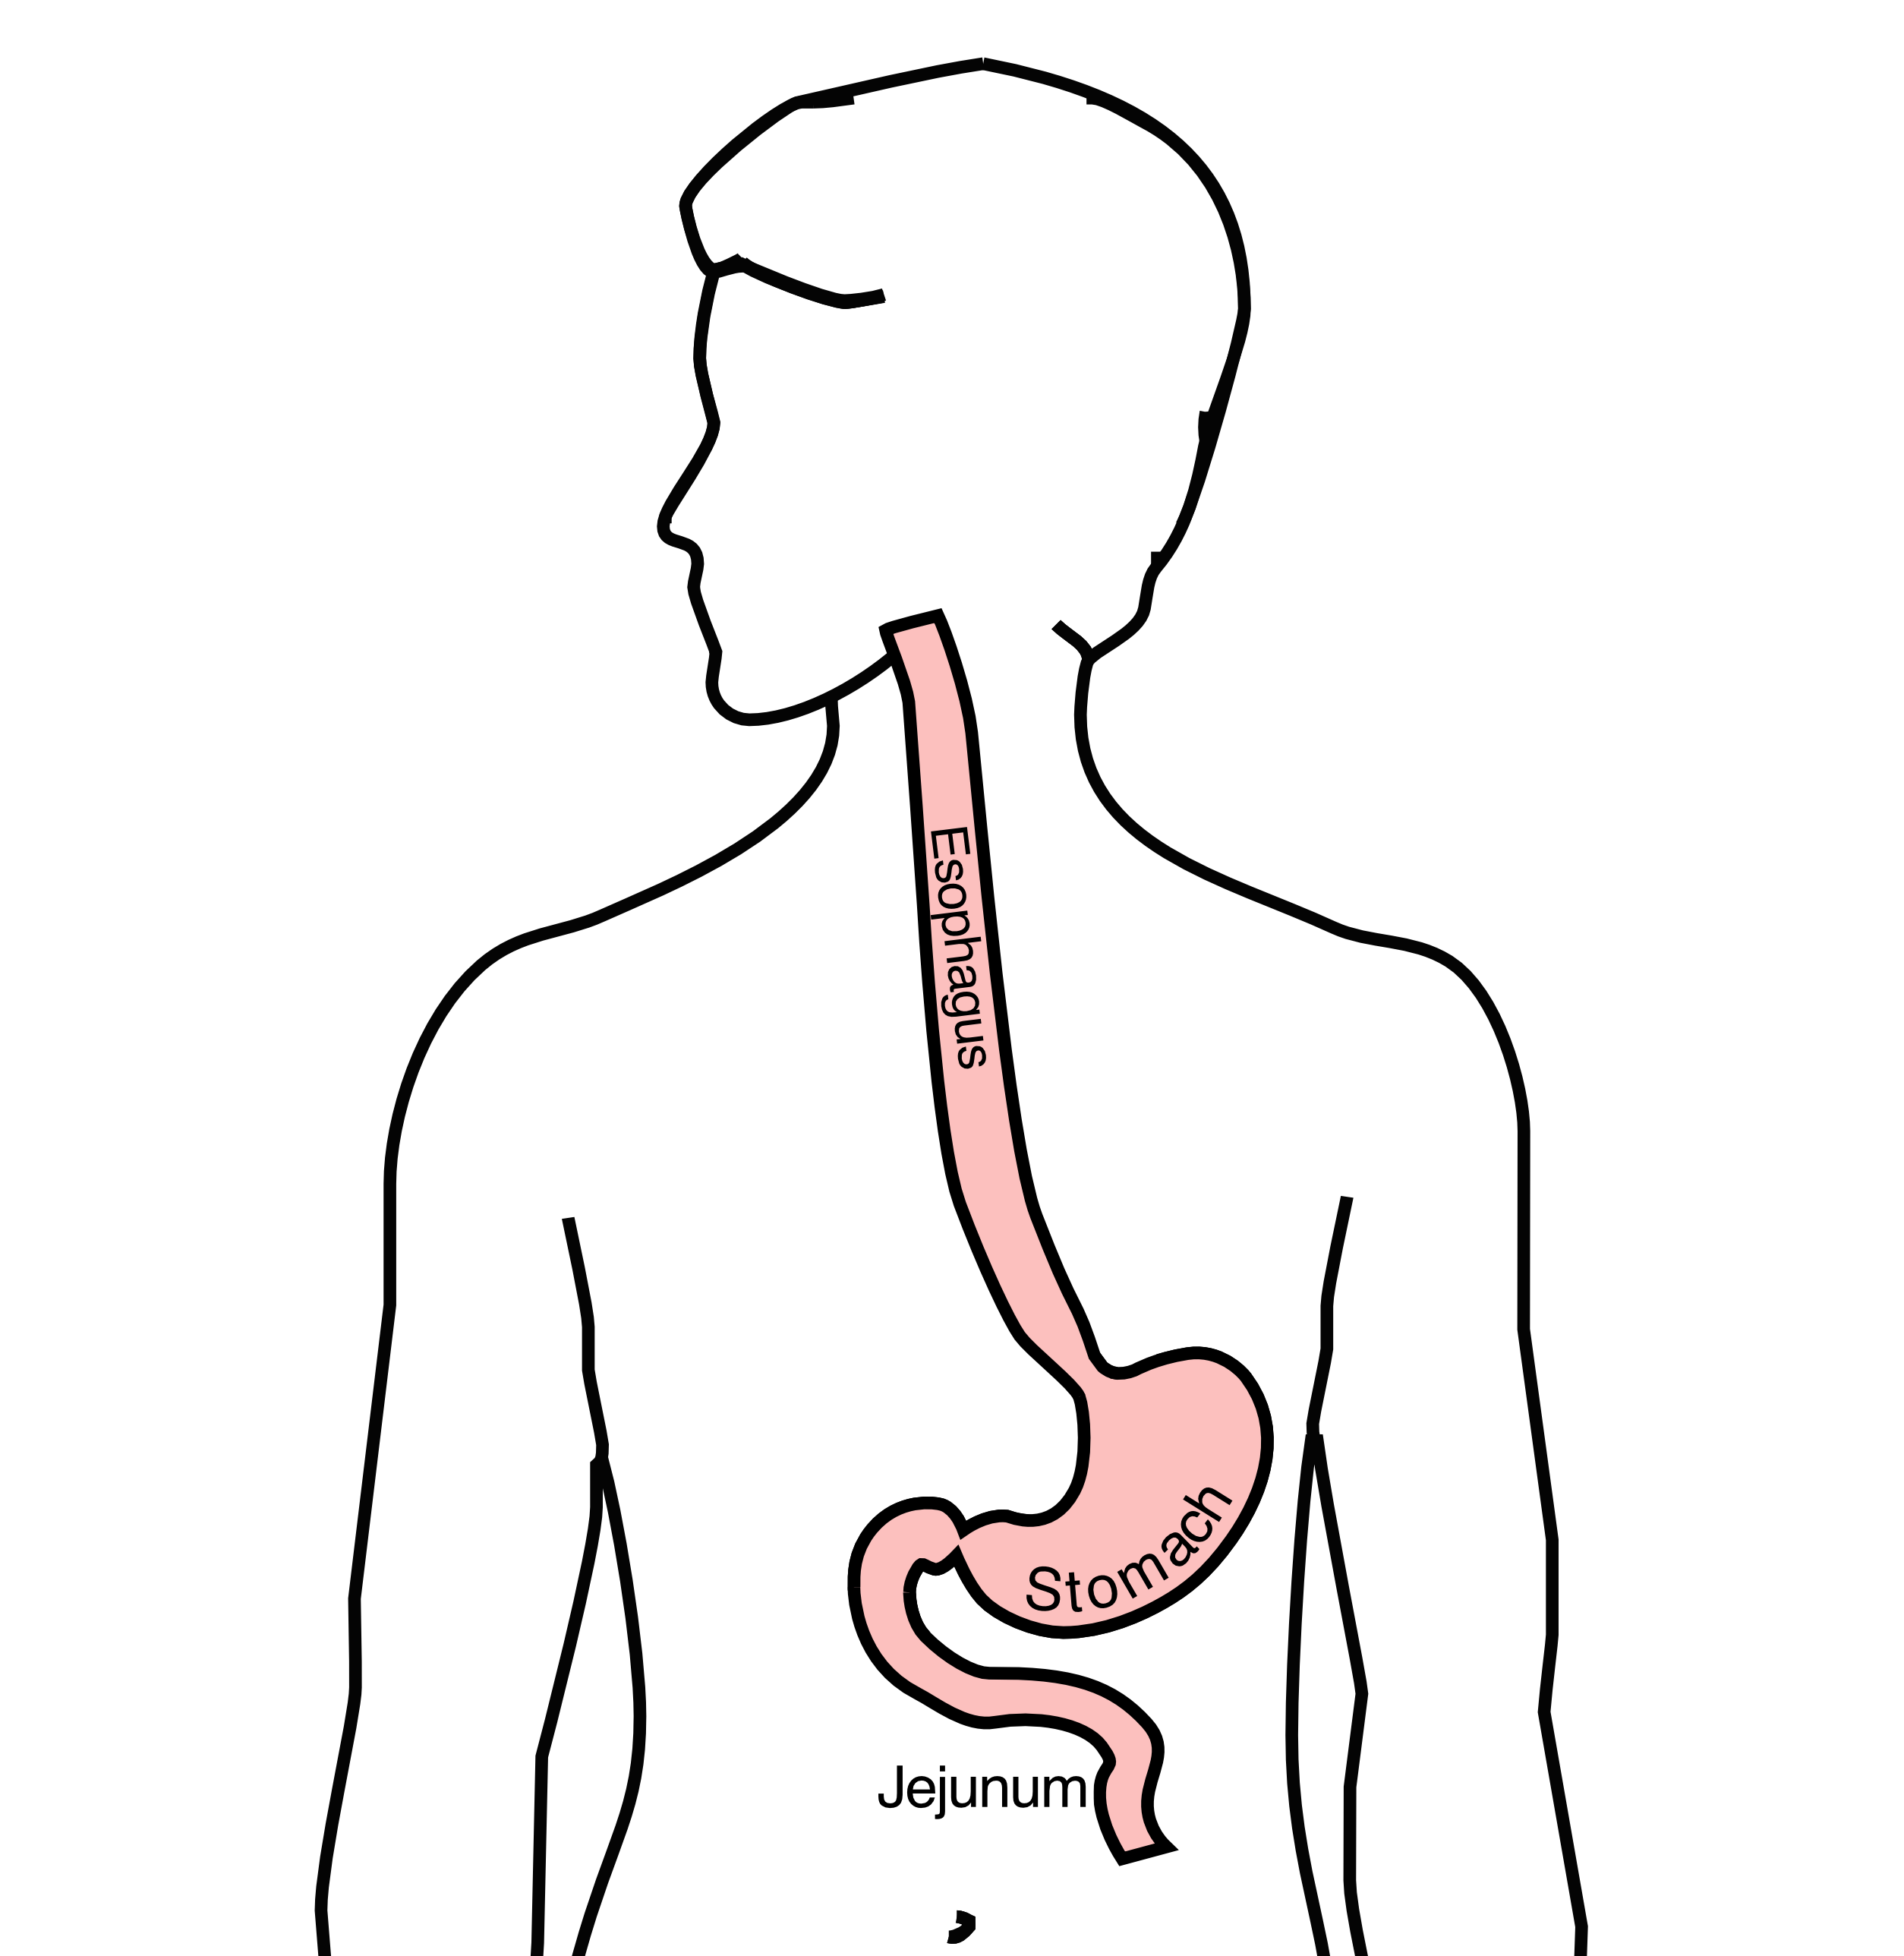
\includegraphics{christmas2004_files/mediabag/Eso_Anatomy_Labels.png}{]}

\subsection{Types of Esophageal
Cancer}\label{types-of-esophageal-cancer}

There are two common types of esophageal cancer

\begin{itemize}
\tightlist
\item
  Adenocarcinoma
\item
  Squamous Cell Carcinoma
\end{itemize}

In many ways, these to different types of esophageal cancer behave the
same.

We will see later in this video, however, that the treatment
\textbf{can} be different depending upon whether the cancer is
adenocarcinoma or squamous cell carcinoma.

\subsection{Cancer Staging}\label{cancer-staging}

Staging refers to the tests to determine

\begin{itemize}
\tightlist
\item
  How large is the tumor?
\item
  Has there been spread to lymph nodes?
\item
  Has it spread to other parts of the body?
\end{itemize}

\textbf{Treatment options depend upont the cancer stage}

\subsection{Esophageal Cancer Staging}\label{esophageal-cancer-staging}

\begin{itemize}
\tightlist
\item
  \textbf{T} = Tumor - How deep has cancer grown into the wall of the
  esophagus?
\item
  \textbf{N} = Nodes - Has cancer spread to the lymph nodes?
\item
  \textbf{M} = Metastasis - Has the cancer spread to other parts of the
  body? lungs or liver?
\end{itemize}

\subsection{Layers of the Wall of the
Esophagus}\label{layers-of-the-wall-of-the-esophagus}

\begin{itemize}
\tightlist
\item
  Mucosa - Inner layer
\item
  Muscle Wall (muscularis)
\item
  Lymph nodes located in fat outside the muscle
\end{itemize}

\includegraphics{christmas2004_files/mediabag/tumor1_ai.png}

\subsection{Early Stage Cancers}\label{early-stage-cancers}

Cancers start on the very inside of the layer called the mucosa

\includegraphics{christmas2004_files/mediabag/tumor21_ai.png}

\subsection{Locally-advanced Cancers}\label{locally-advanced-cancers}

Over time, cancers can grow into the muscular wall

\includegraphics{christmas2004_files/mediabag/tumor24_ai.png}

\subsection{Lymph Nodes}\label{lymph-nodes}

In some cases, cancer cells can break off from the main tumor and spread
to lymph nodes

\includegraphics{christmas2004_files/mediabag/tumor25b_ai.png}

\subsection{T Stage}\label{t-stage}

Cancers are categorized based upon the thickness of the tumor, known as
the T stage

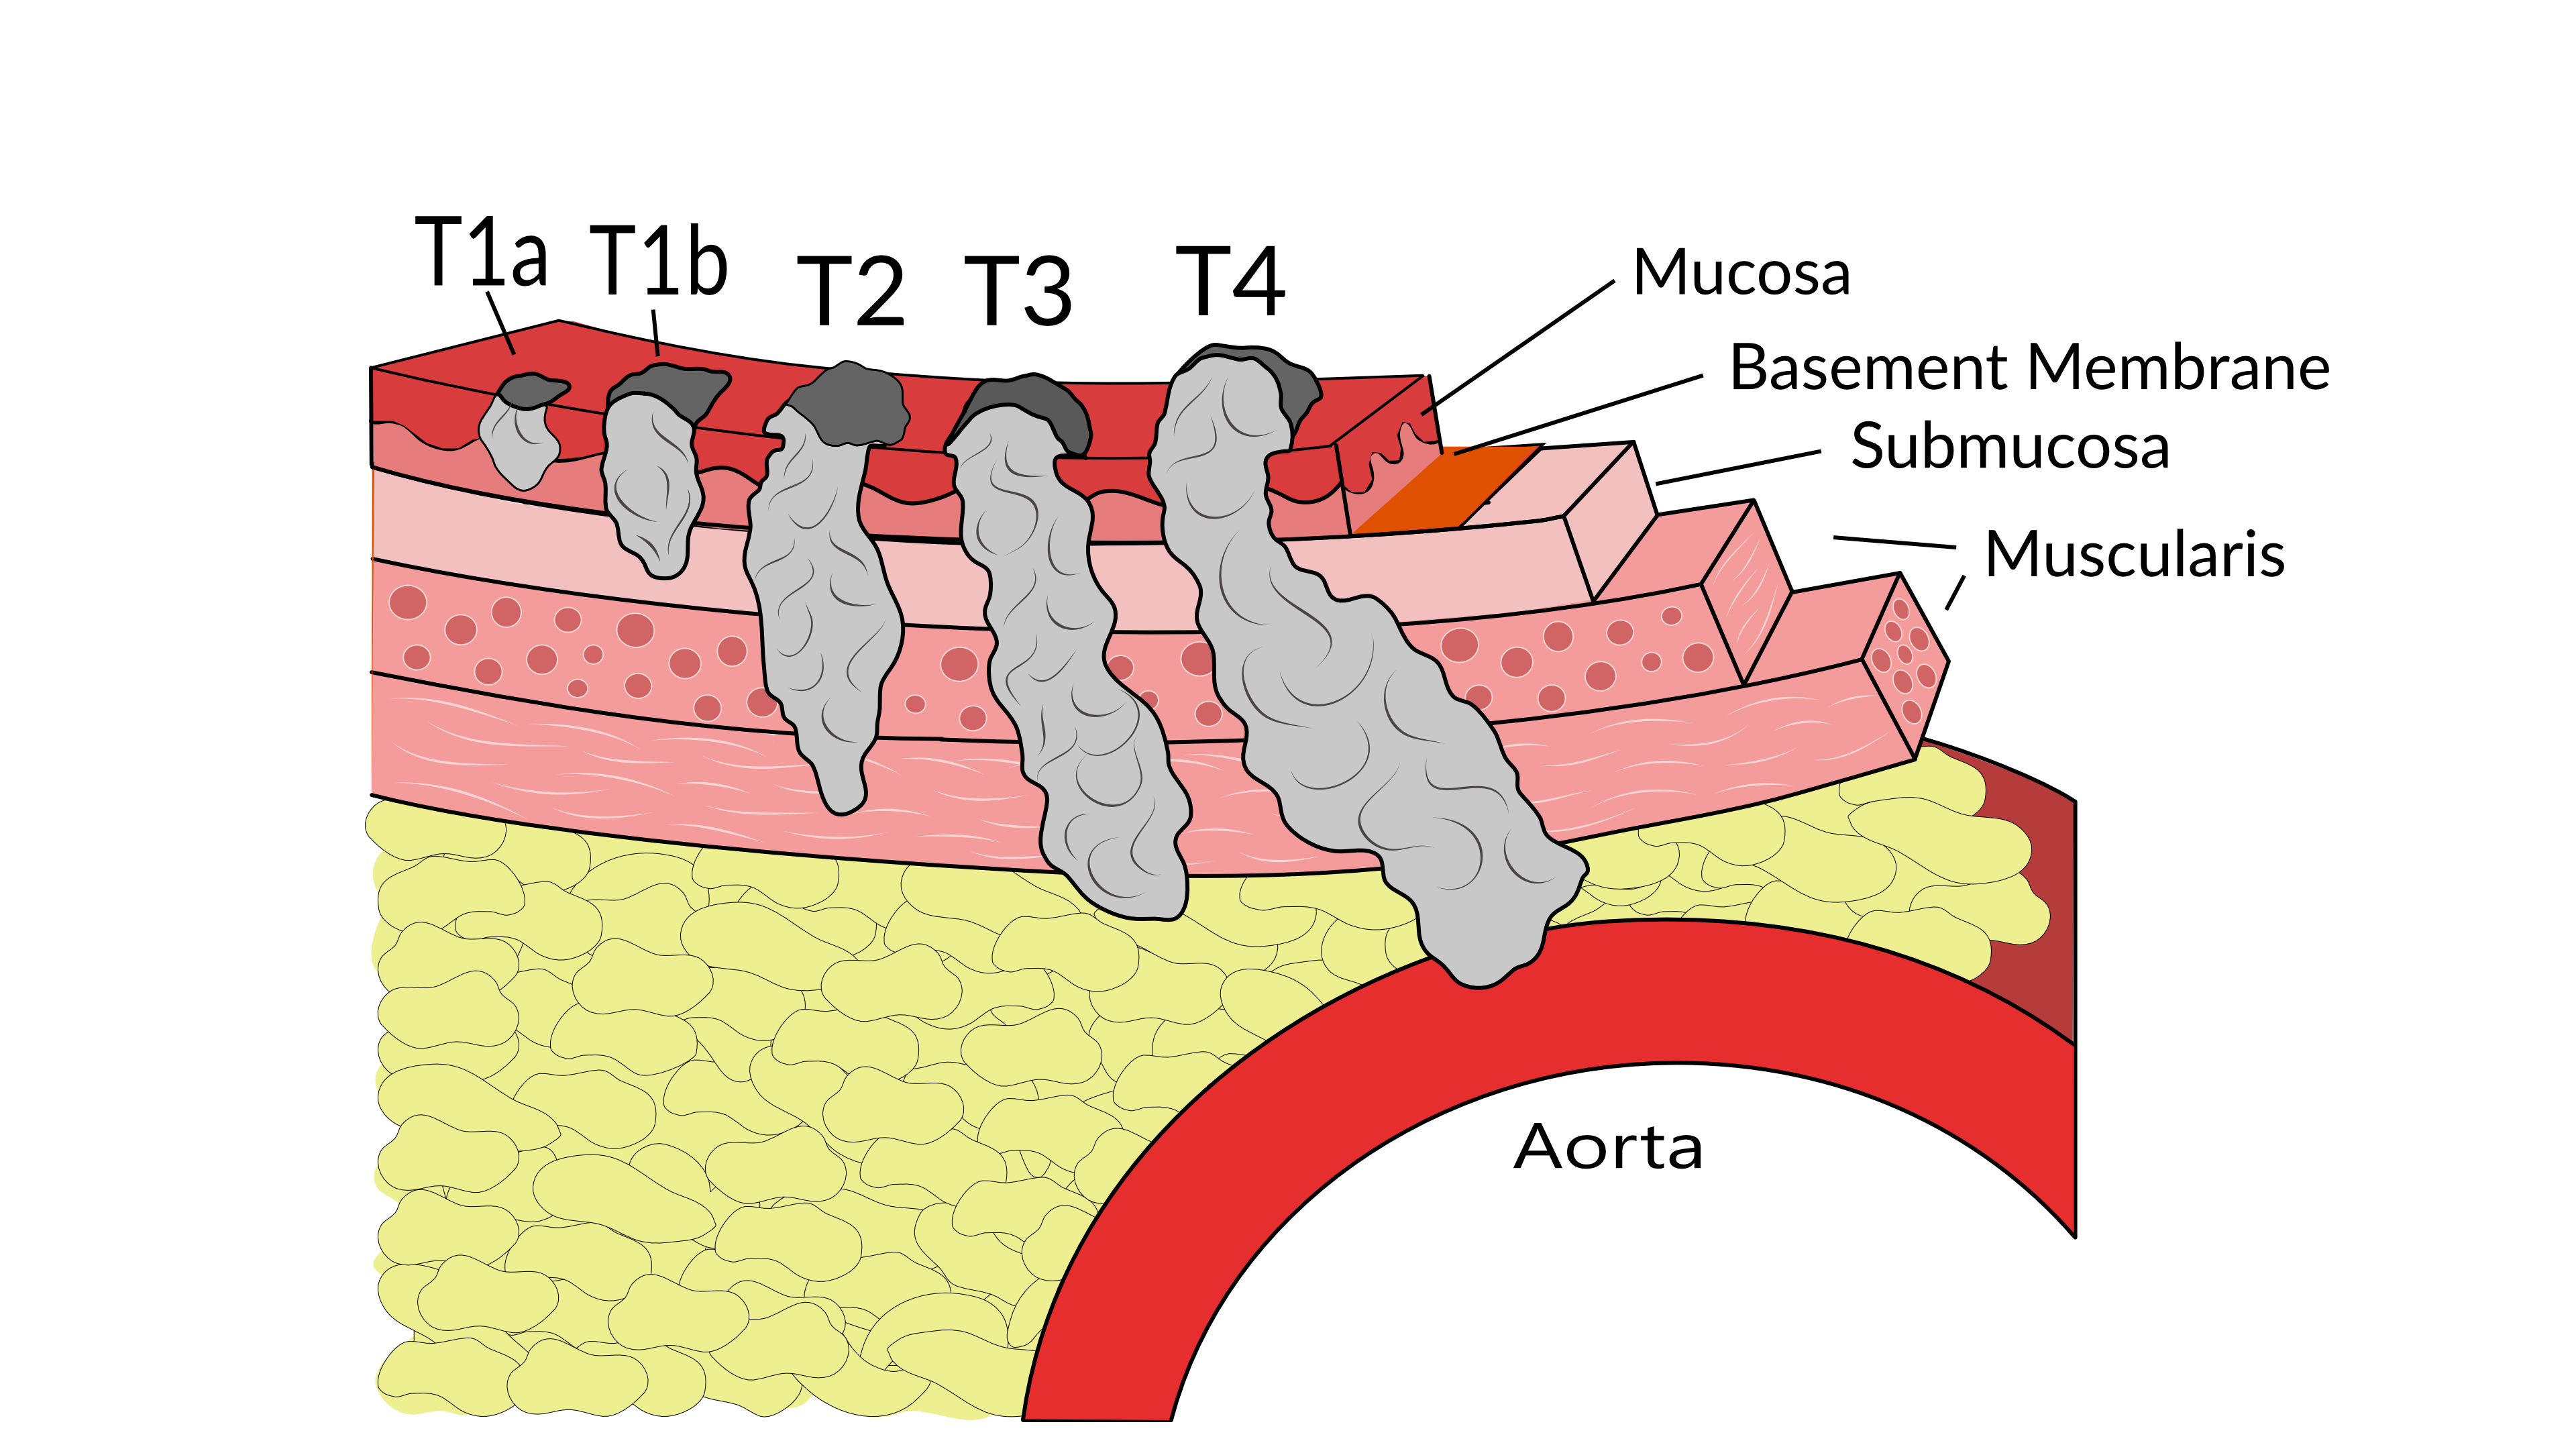
\includegraphics{christmas2004_files/mediabag/tumor_t_full.png}

\subsection{N Stage}\label{n-stage}

Cancers are categorized by whether there is spread to the lymph nodes.

\begin{itemize}
\tightlist
\item
  \textbf{N0} cancers have not spread to the lymph nodes
\item
  \textbf{N1} cancers have spread to the lymph nodes.
\end{itemize}

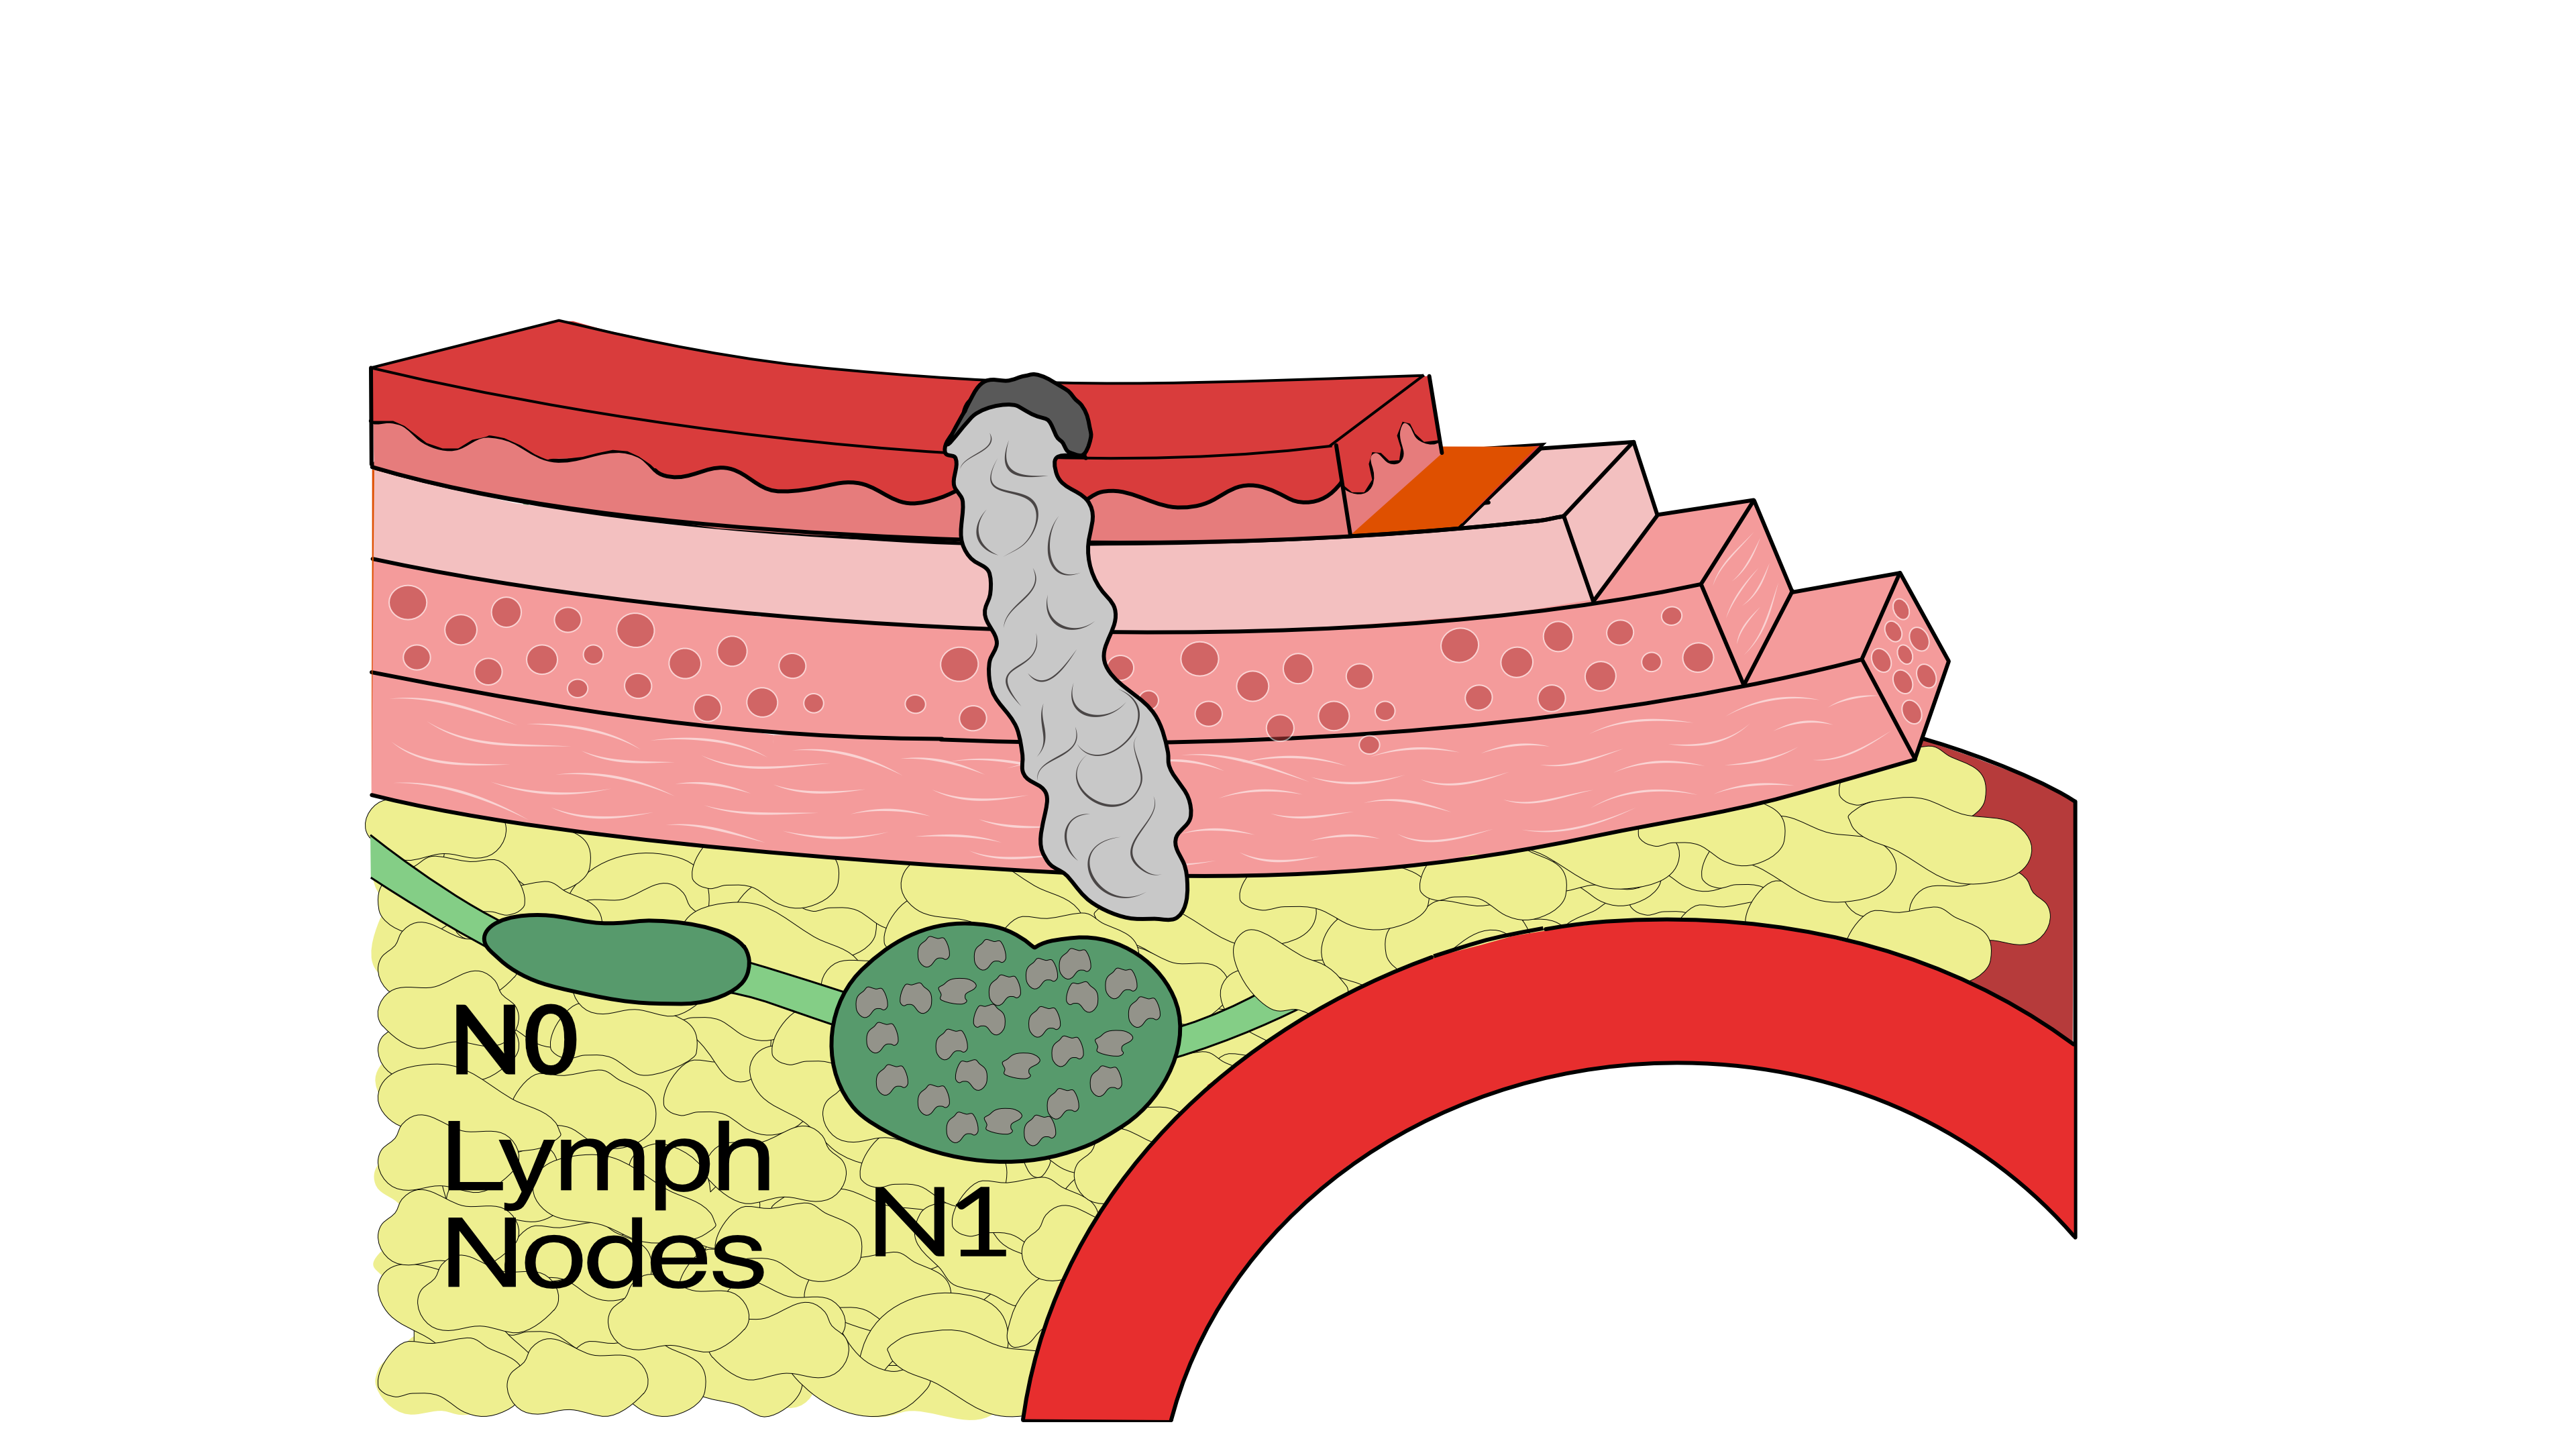
\includegraphics{christmas2004_files/mediabag/tumor_t3_nodes_label.png}

\subsection{M Stage}\label{m-stage}

Some cancers can also spread from the esophagus to the lungs or liver

\begin{itemize}
\tightlist
\item
  \textbf{M0} cancers have not spread to other parts of the body
\item
  \textbf{N1} cancers have spread to other parts of the body such as
  lungs or liver
\end{itemize}

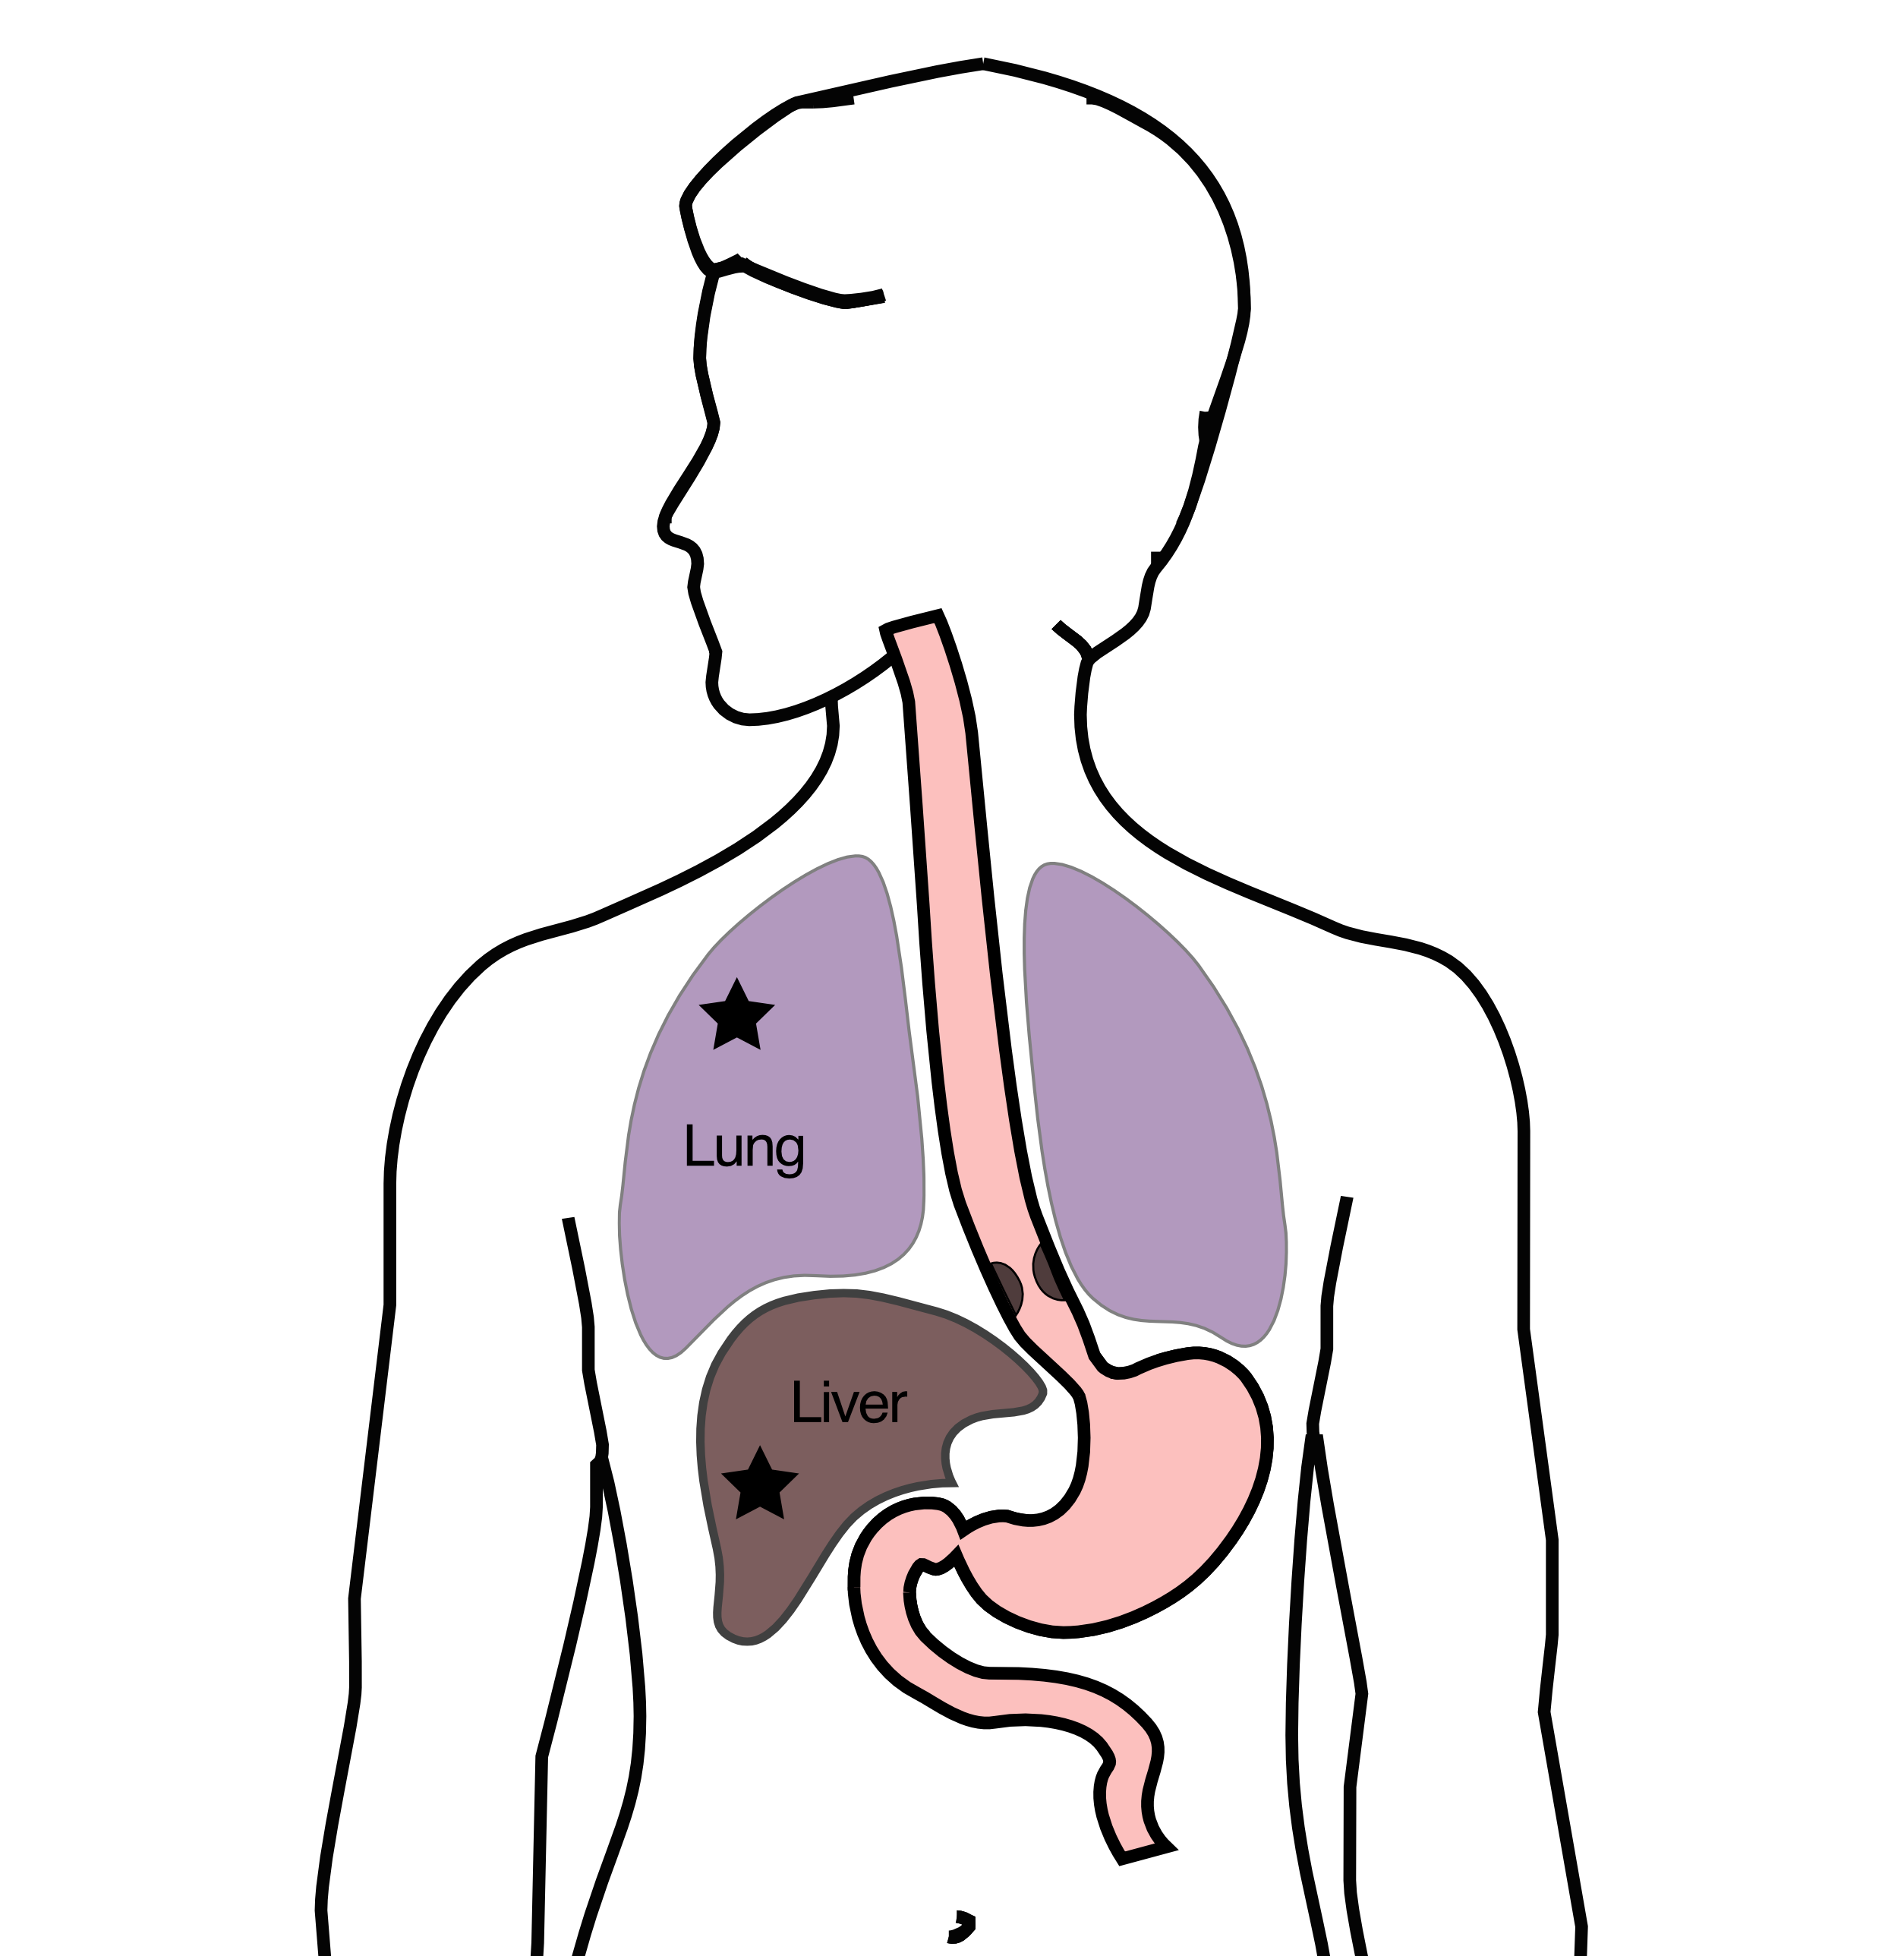
\includegraphics{christmas2004_files/mediabag/Eso_M_Stage.png}

\subsection{PET scan}\label{pet-scan}

A PET scan is similar to a CT scan, and uses a small amount of tracer to
light up areas of cancer.

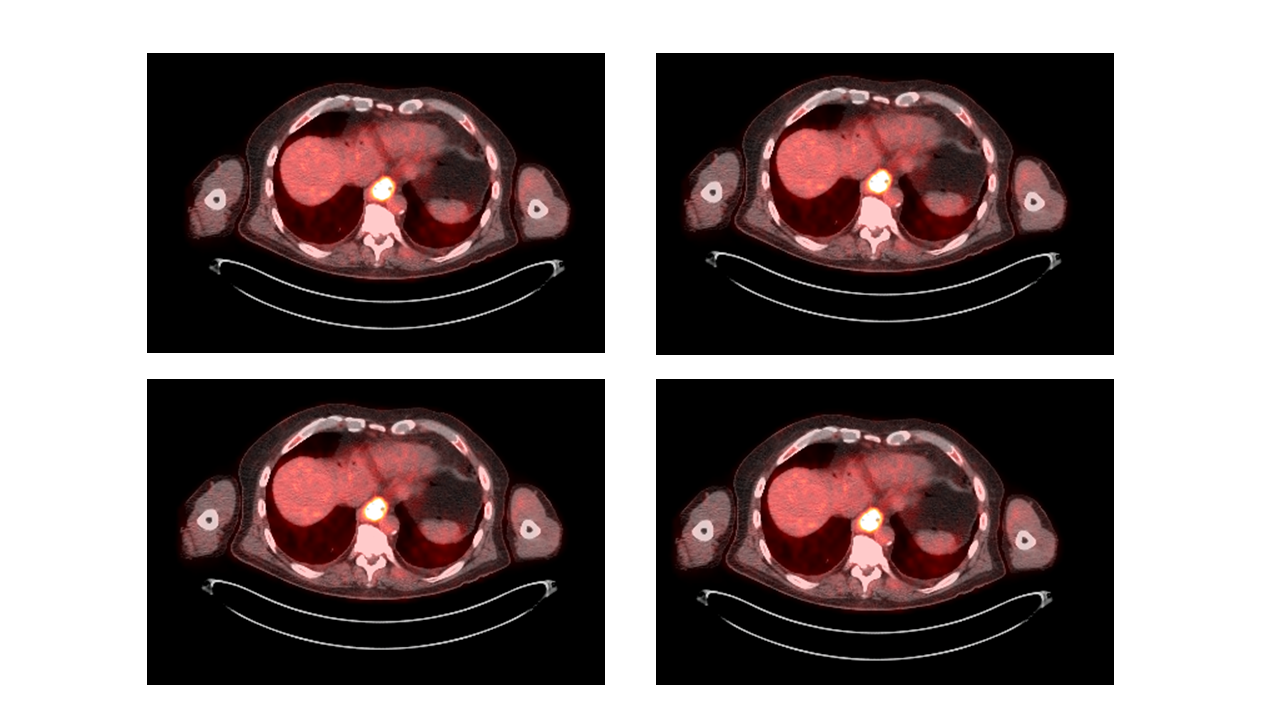
\includegraphics{christmas2004_files/mediabag/PetImage.png}

\subsection{Endoscopic Ultrasound}\label{endoscopic-ultrasound}

Endoscopic ultrasound (EUS) is a procedure similar to upper endoscopy
(EGD) which has an ultrasound probe at the bottom of the scope. This
allows measuring the thickness of the cancer. Endoscopic ultrasound can
help determine the T stage of the cancer.

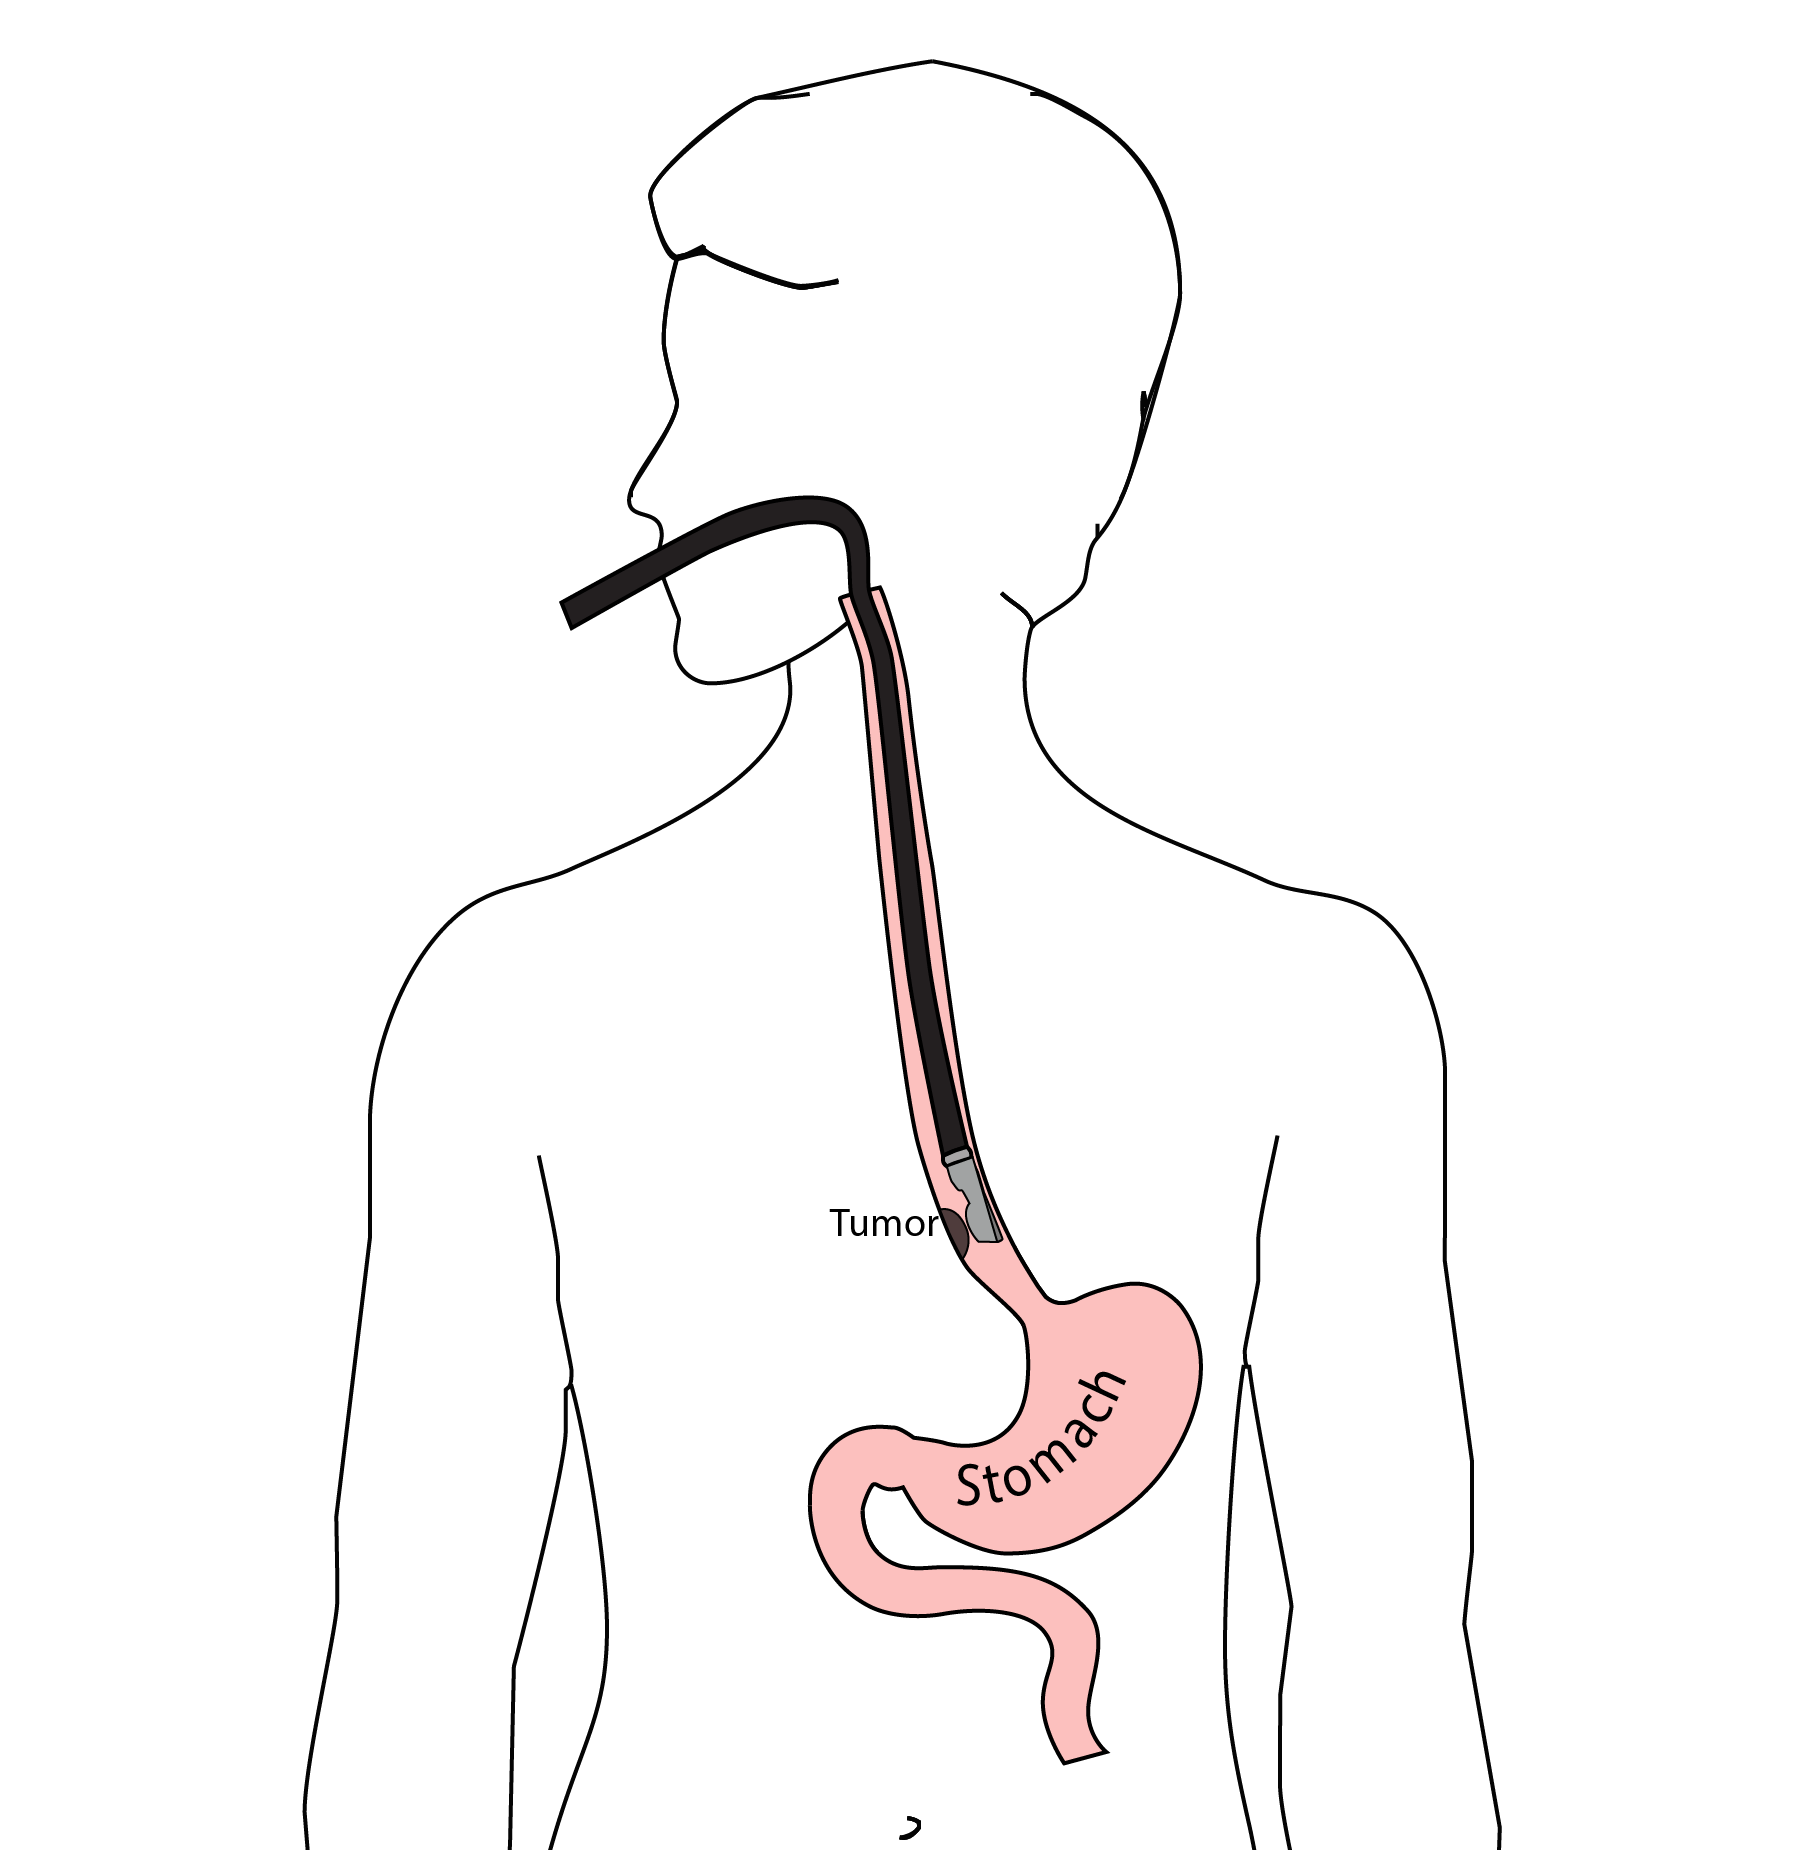
\includegraphics{christmas2004_files/mediabag/EUSArtboard.png}

\subsection{Laparoscopy}\label{laparoscopy}

Some esophageal cancers can spread inside the abdominal cavity. These
areas of spread can be very small, as small as a grain of rice.

In order to detect spread within the abdominal cavity, a proceduce
called a laparoscopy can be performed in some some patients.

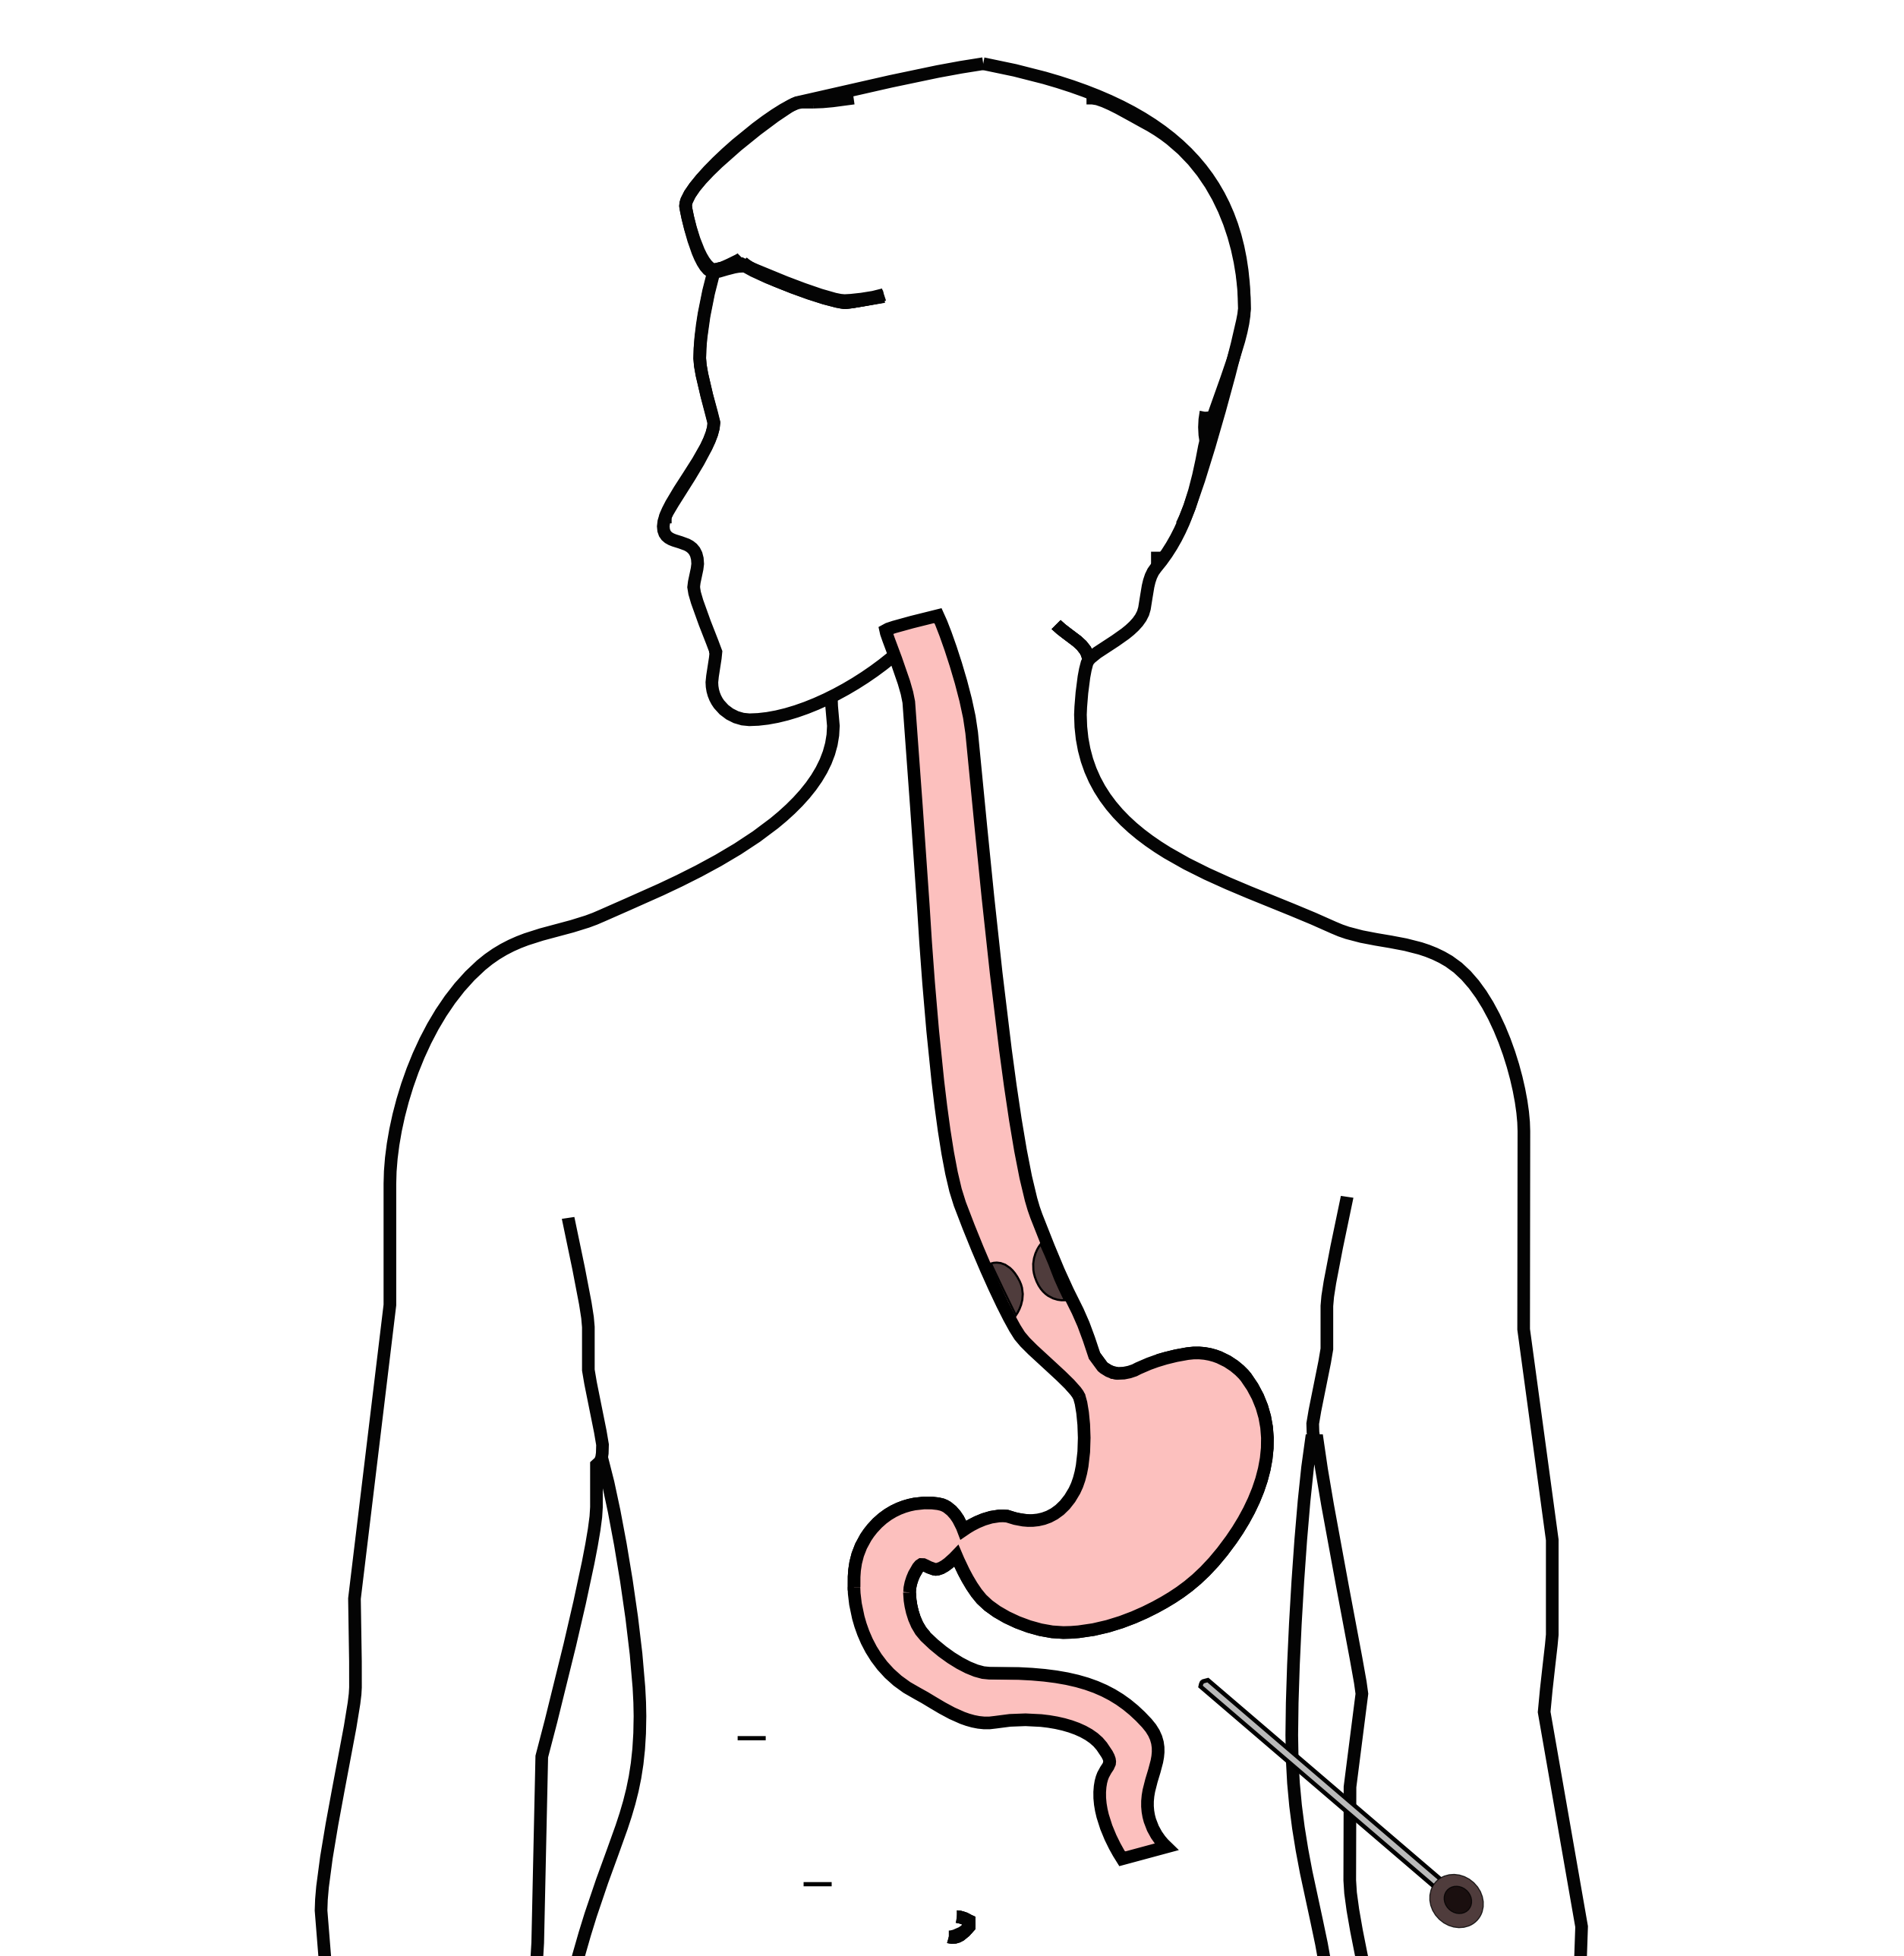
\includegraphics{christmas2004_files/mediabag/Eso_Laparoscopy.png}

\subsection{Laparoscopy}\label{laparoscopy-1}

A laparoscopy is performed under a general anesthetic.

\begin{itemize}
\tightlist
\item
  Several incisions 1/4'' long
\item
  A telescope is inserted to look inside the abdominal cavity.
\item
  Biopsies can be performed.
\end{itemize}

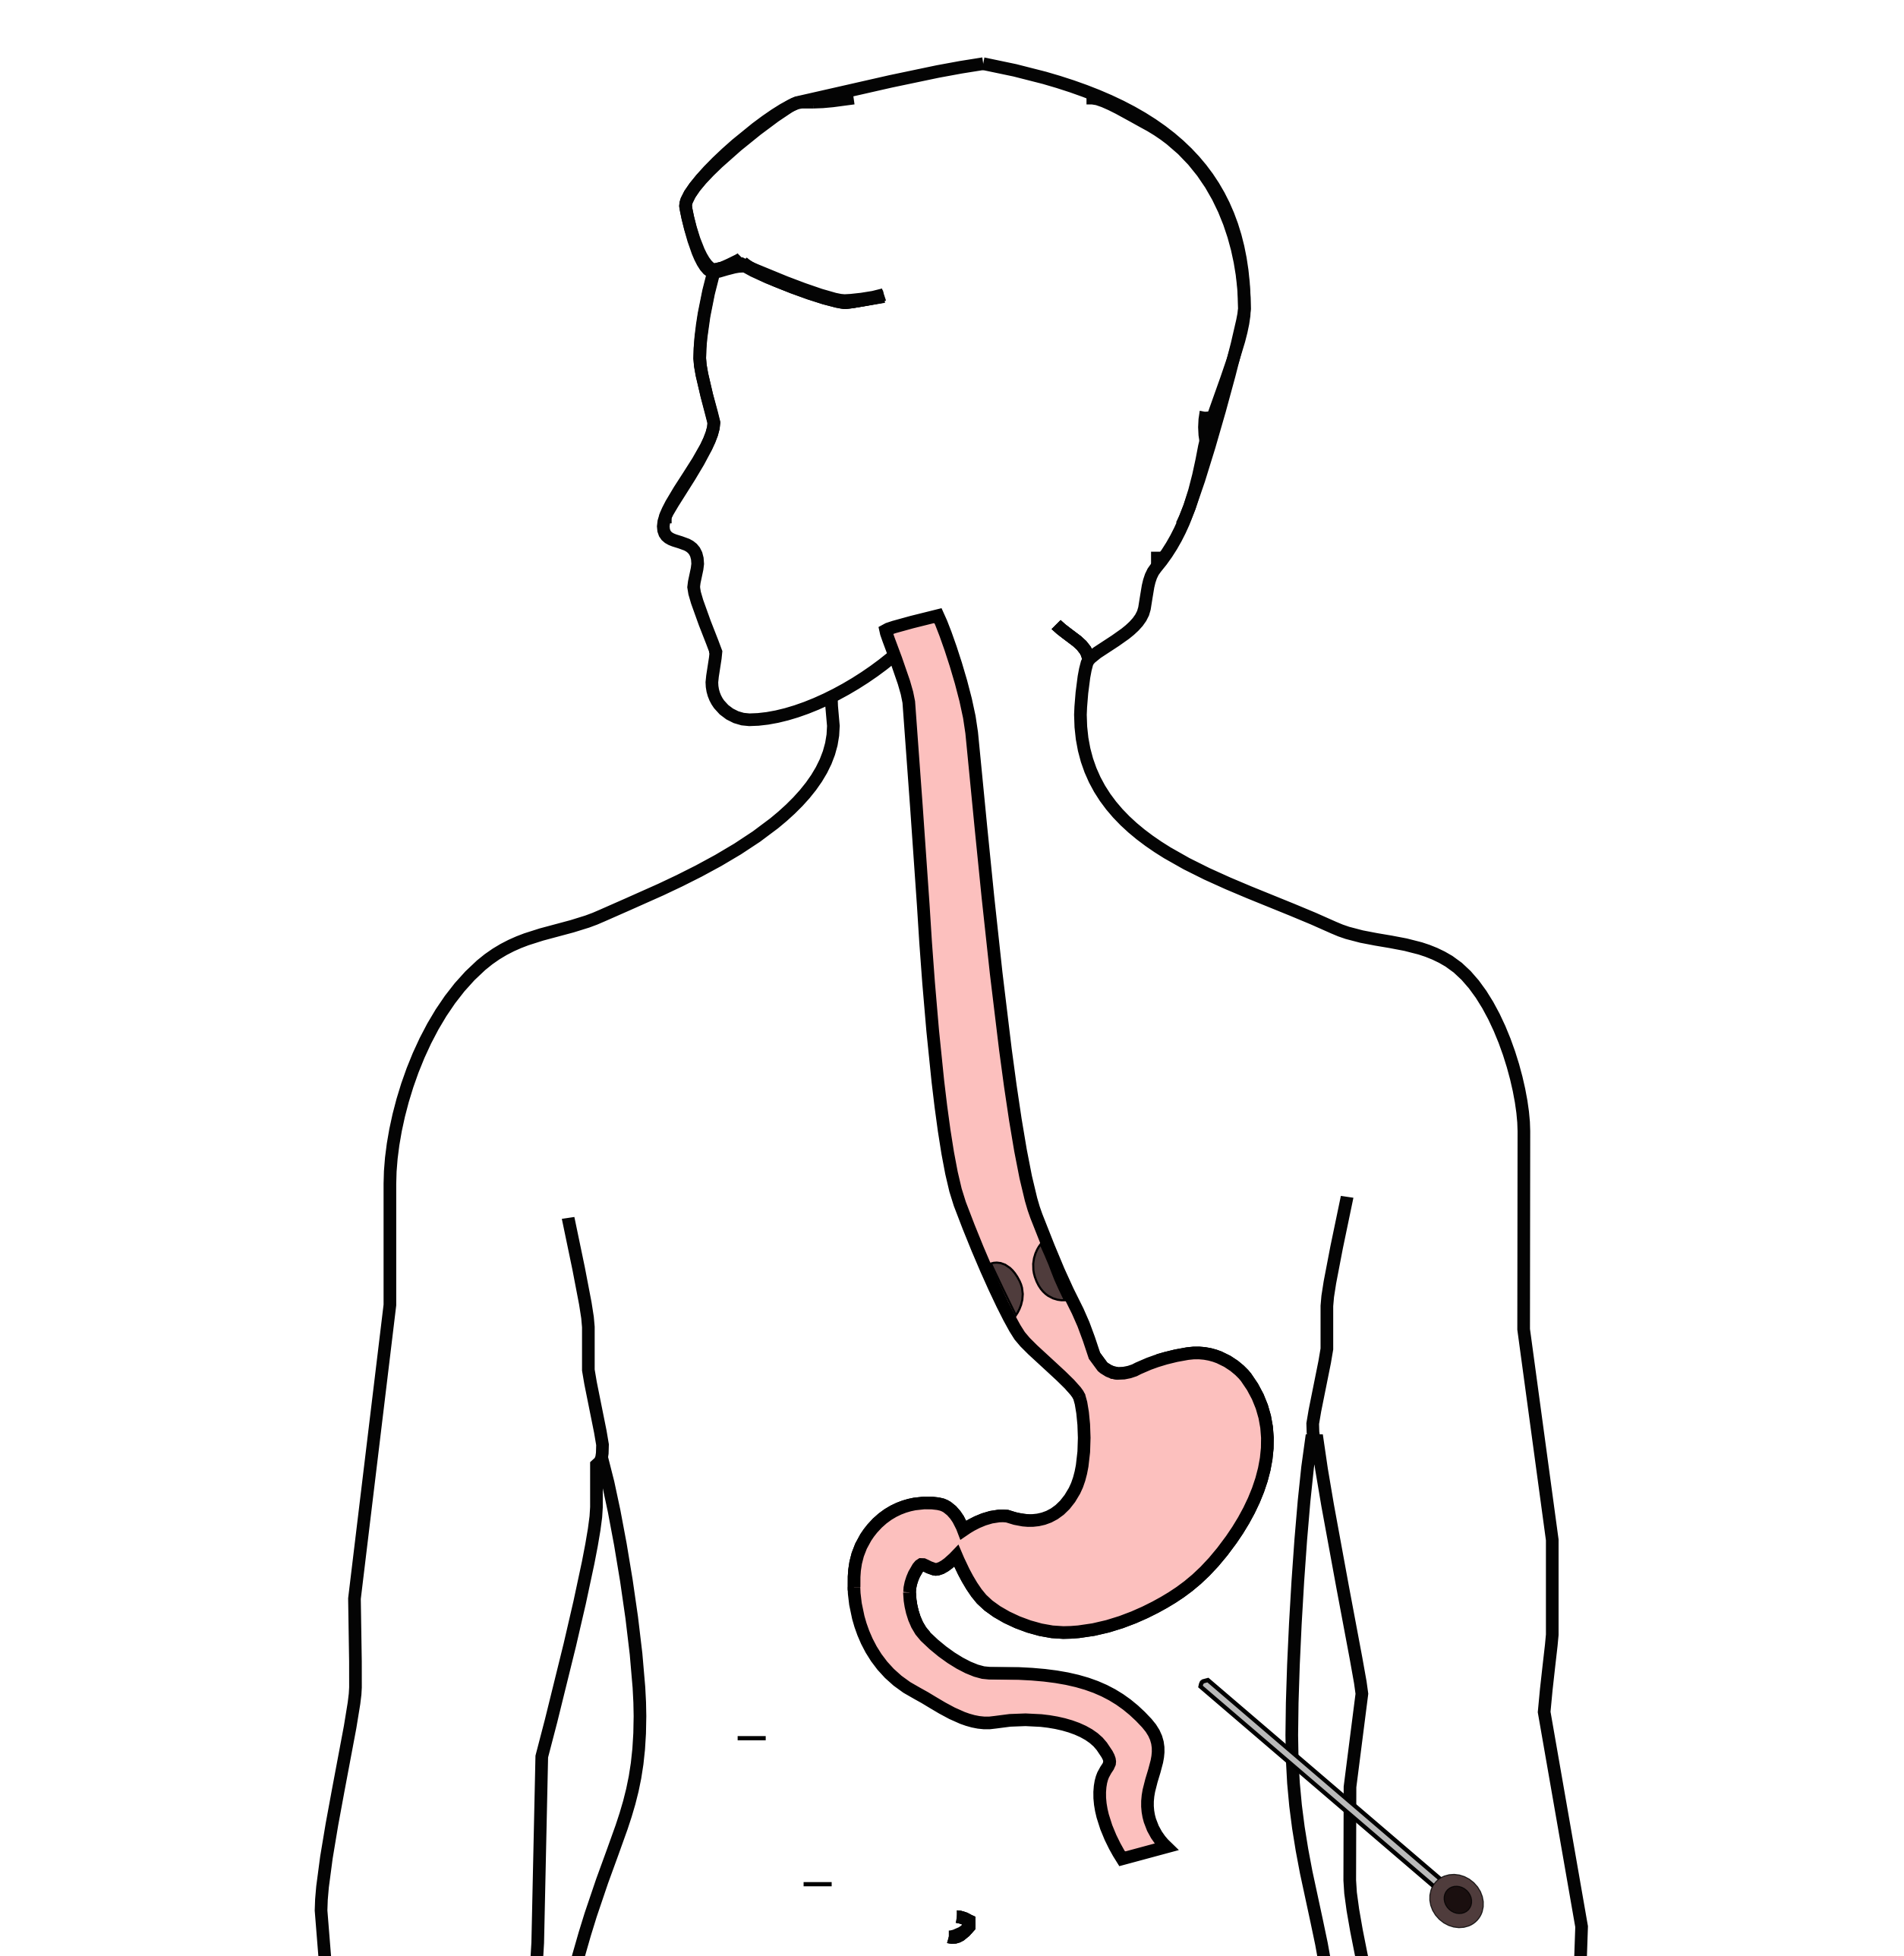
\includegraphics{christmas2004_files/mediabag/Eso_Laparoscopy.png}

\subsection{Treatment Plans}\label{treatment-plans}

\begin{itemize}
\tightlist
\item
  Superficial (T1) \(\Rightarrow\) Endoscopic Therapy
\item
  Localized (T1b/T2) \(\Rightarrow\) Surgery
\item
  Locally-advanced (T3/N1) \(\Rightarrow\) Chemo \(\pm\) Radiation
  \(\rightarrow\)Surgery
\item
  Metastatic (M1) \(\Rightarrow\) Chemotherapy
\end{itemize}

\subsection{Superficial Cancers}\label{superficial-cancers}

Superficial Cancers = T1a N0

Treatment is often with endoscopy without the need for surgery.

\includegraphics{christmas2004_files/mediabag/tumor21_ai.png}

\subsection{Endoscopic Mucosal Resection
(EMR)}\label{endoscopic-mucosal-resection-emr}

Endoscopic procedure to remove a superficial tumor from the inner layer
of the esophagus

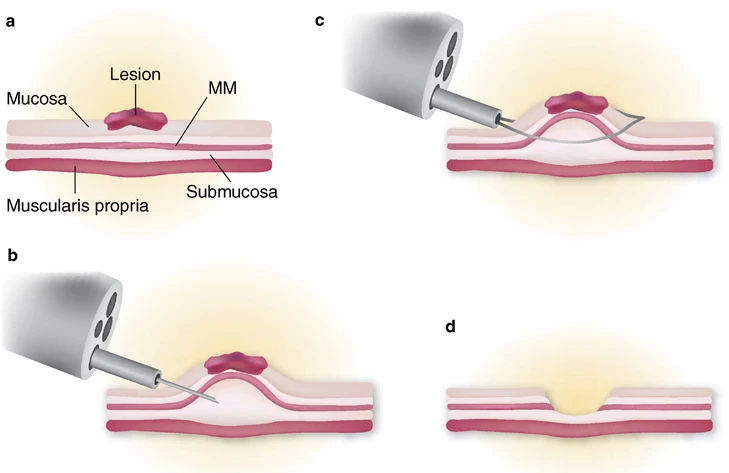
\includegraphics{christmas2004_files/mediabag/emr_comm.png}

\subsection{Endoscopic Mucosal Resection -
Favorable}\label{endoscopic-mucosal-resection---favorable}

\begin{itemize}
\tightlist
\item
  Clear margins at the edge \emph{AND}
\item
  Clear deep margin \emph{AND}
\item
  Tumor appears slow-growing under microscope
\end{itemize}

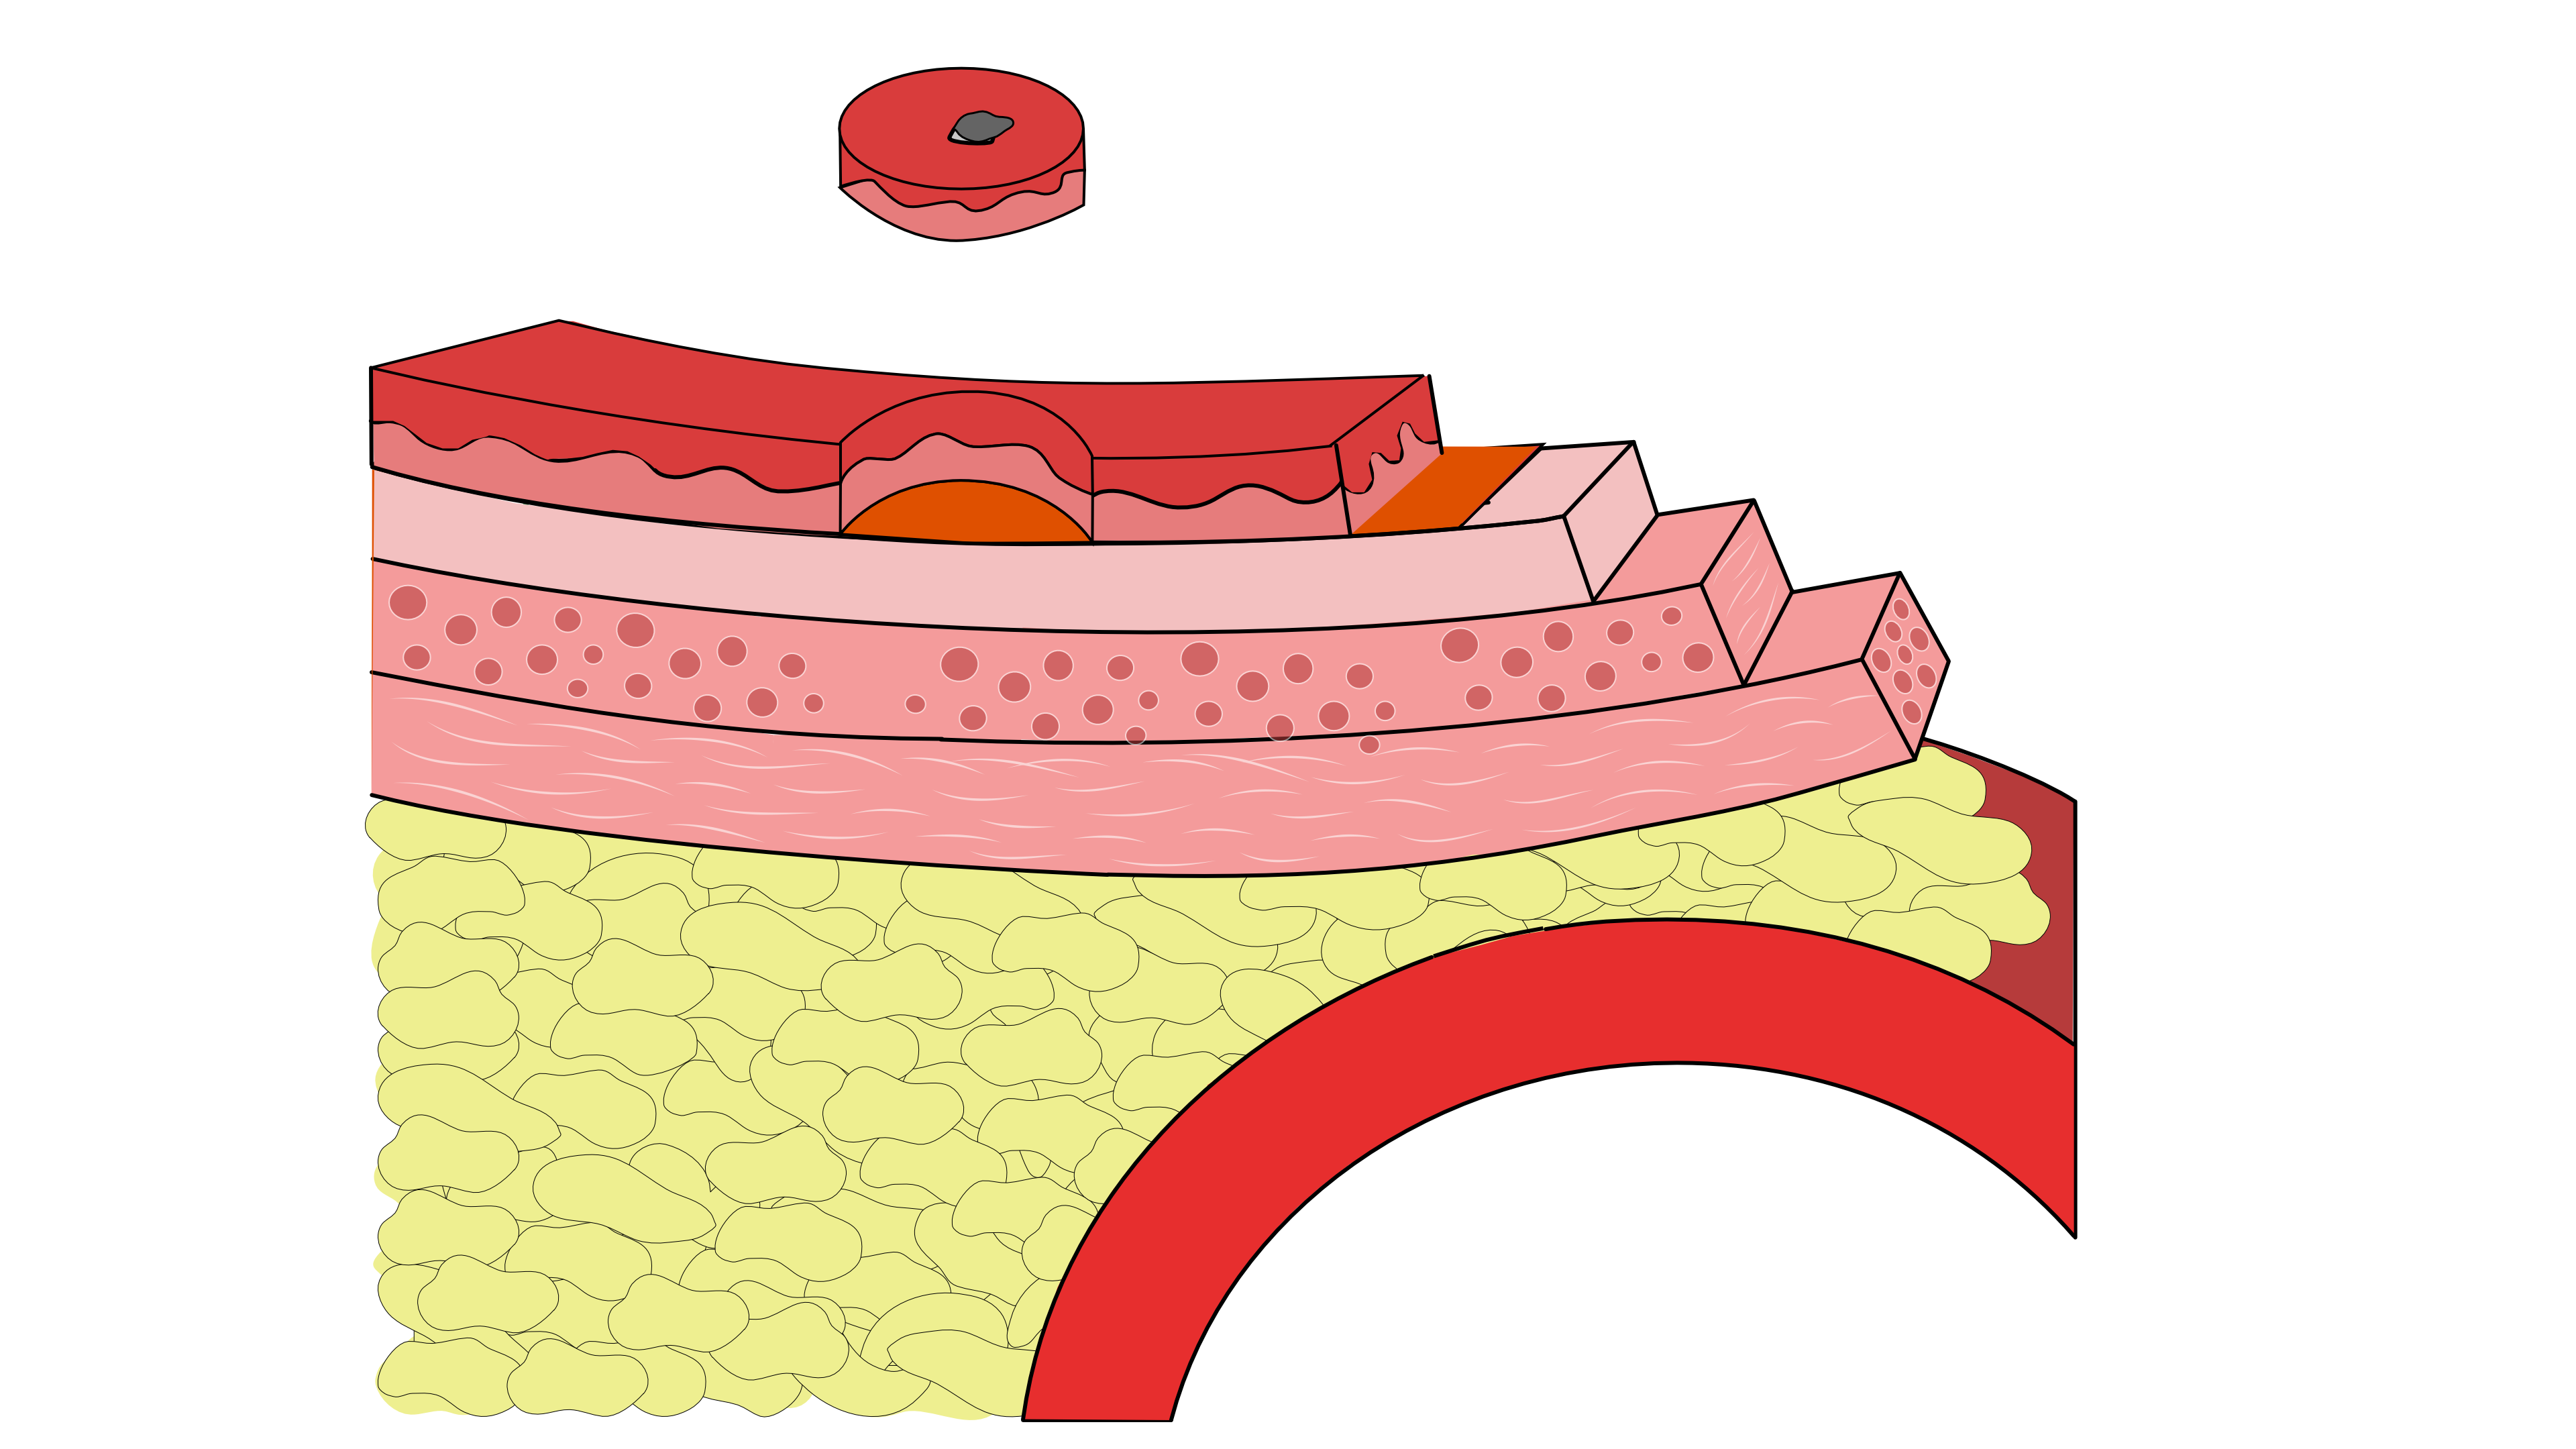
\includegraphics{christmas2004_files/mediabag/emr_favorable.png}

\subsection{Endoscopic Mucosal Resection -
Favorable}\label{endoscopic-mucosal-resection---favorable-1}

\begin{itemize}
\tightlist
\item
  Clear margins at the edge \emph{AND}
\item
  Clear deep margin \emph{AND}
\item
  Tumor appears slow-growing under microscope
\end{itemize}

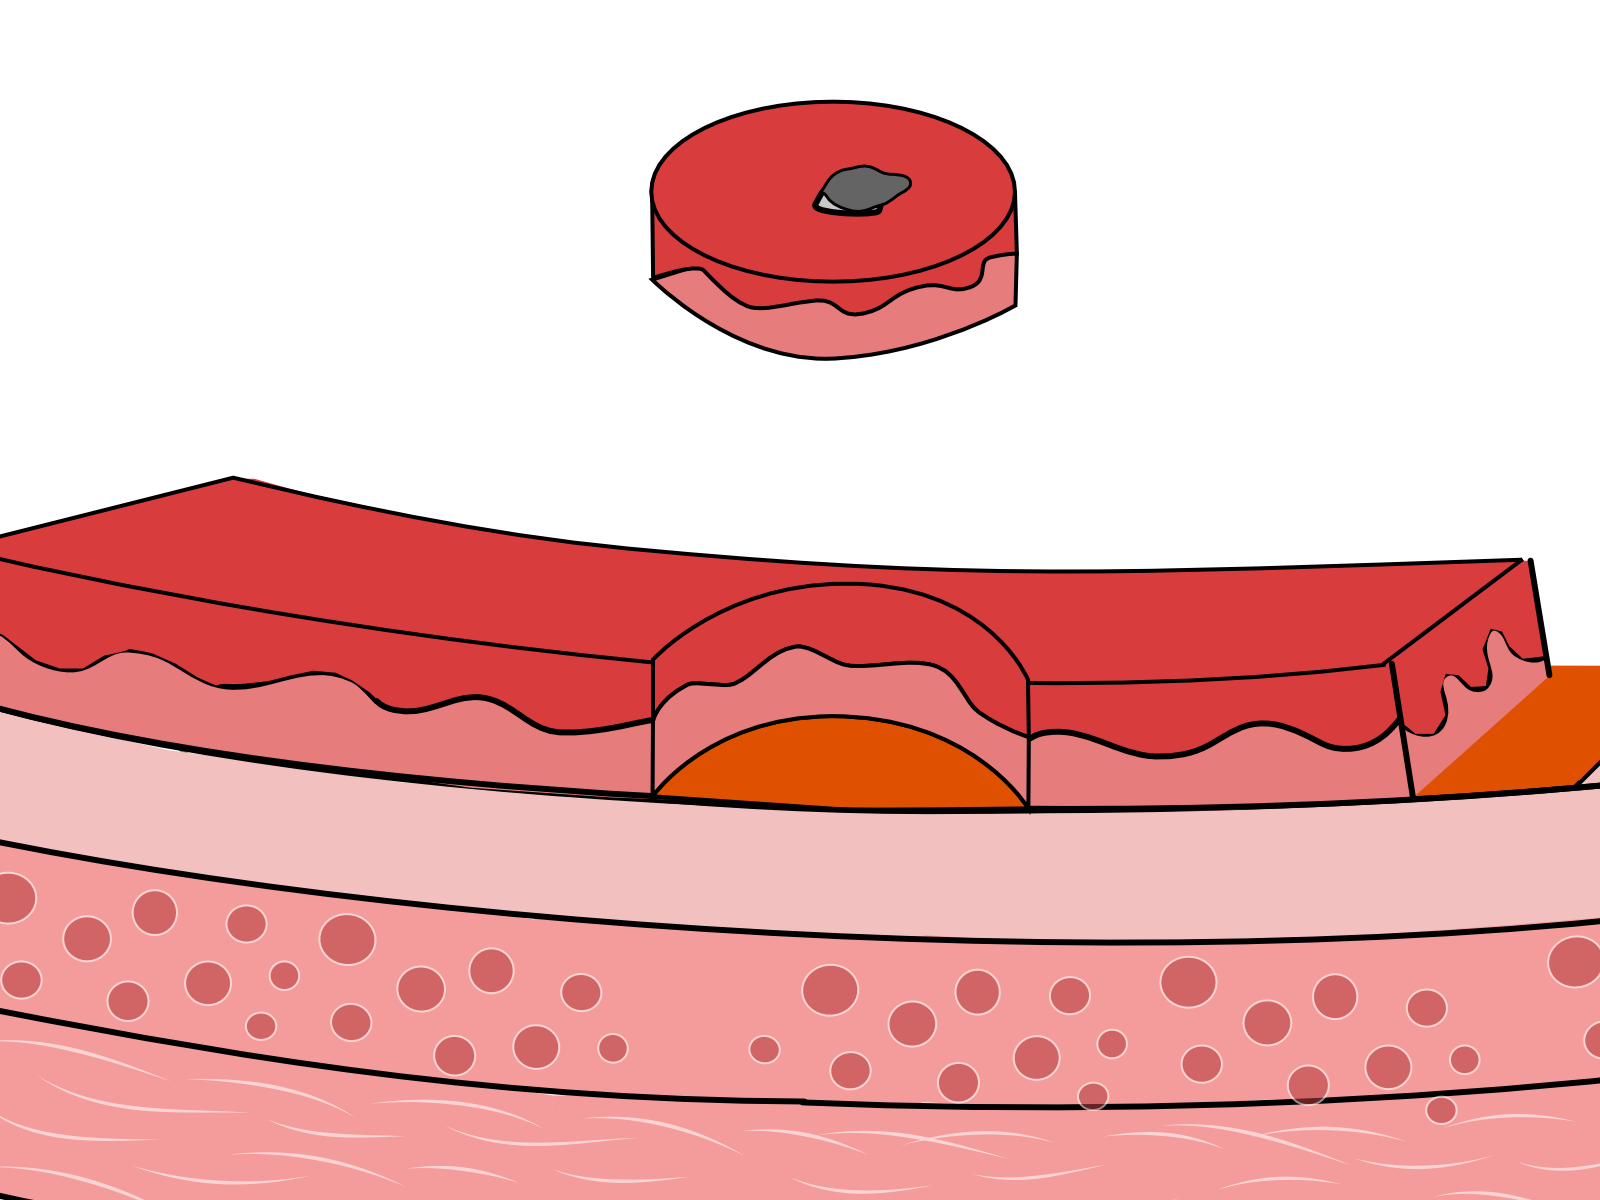
\includegraphics{christmas2004_files/mediabag/emr_favorable_160012.png}

EMR may be sufficient treatment (without surgery)

\subsection{Endoscopic Mucosal Resection -
Unfavorable}\label{endoscopic-mucosal-resection---unfavorable}

\begin{itemize}
\tightlist
\item
  Tumor at edge margin \emph{OR}
\item
  Tumor at deep margin \emph{OR}
\item
  Tumor appears rapidly-growing under microscope
\end{itemize}

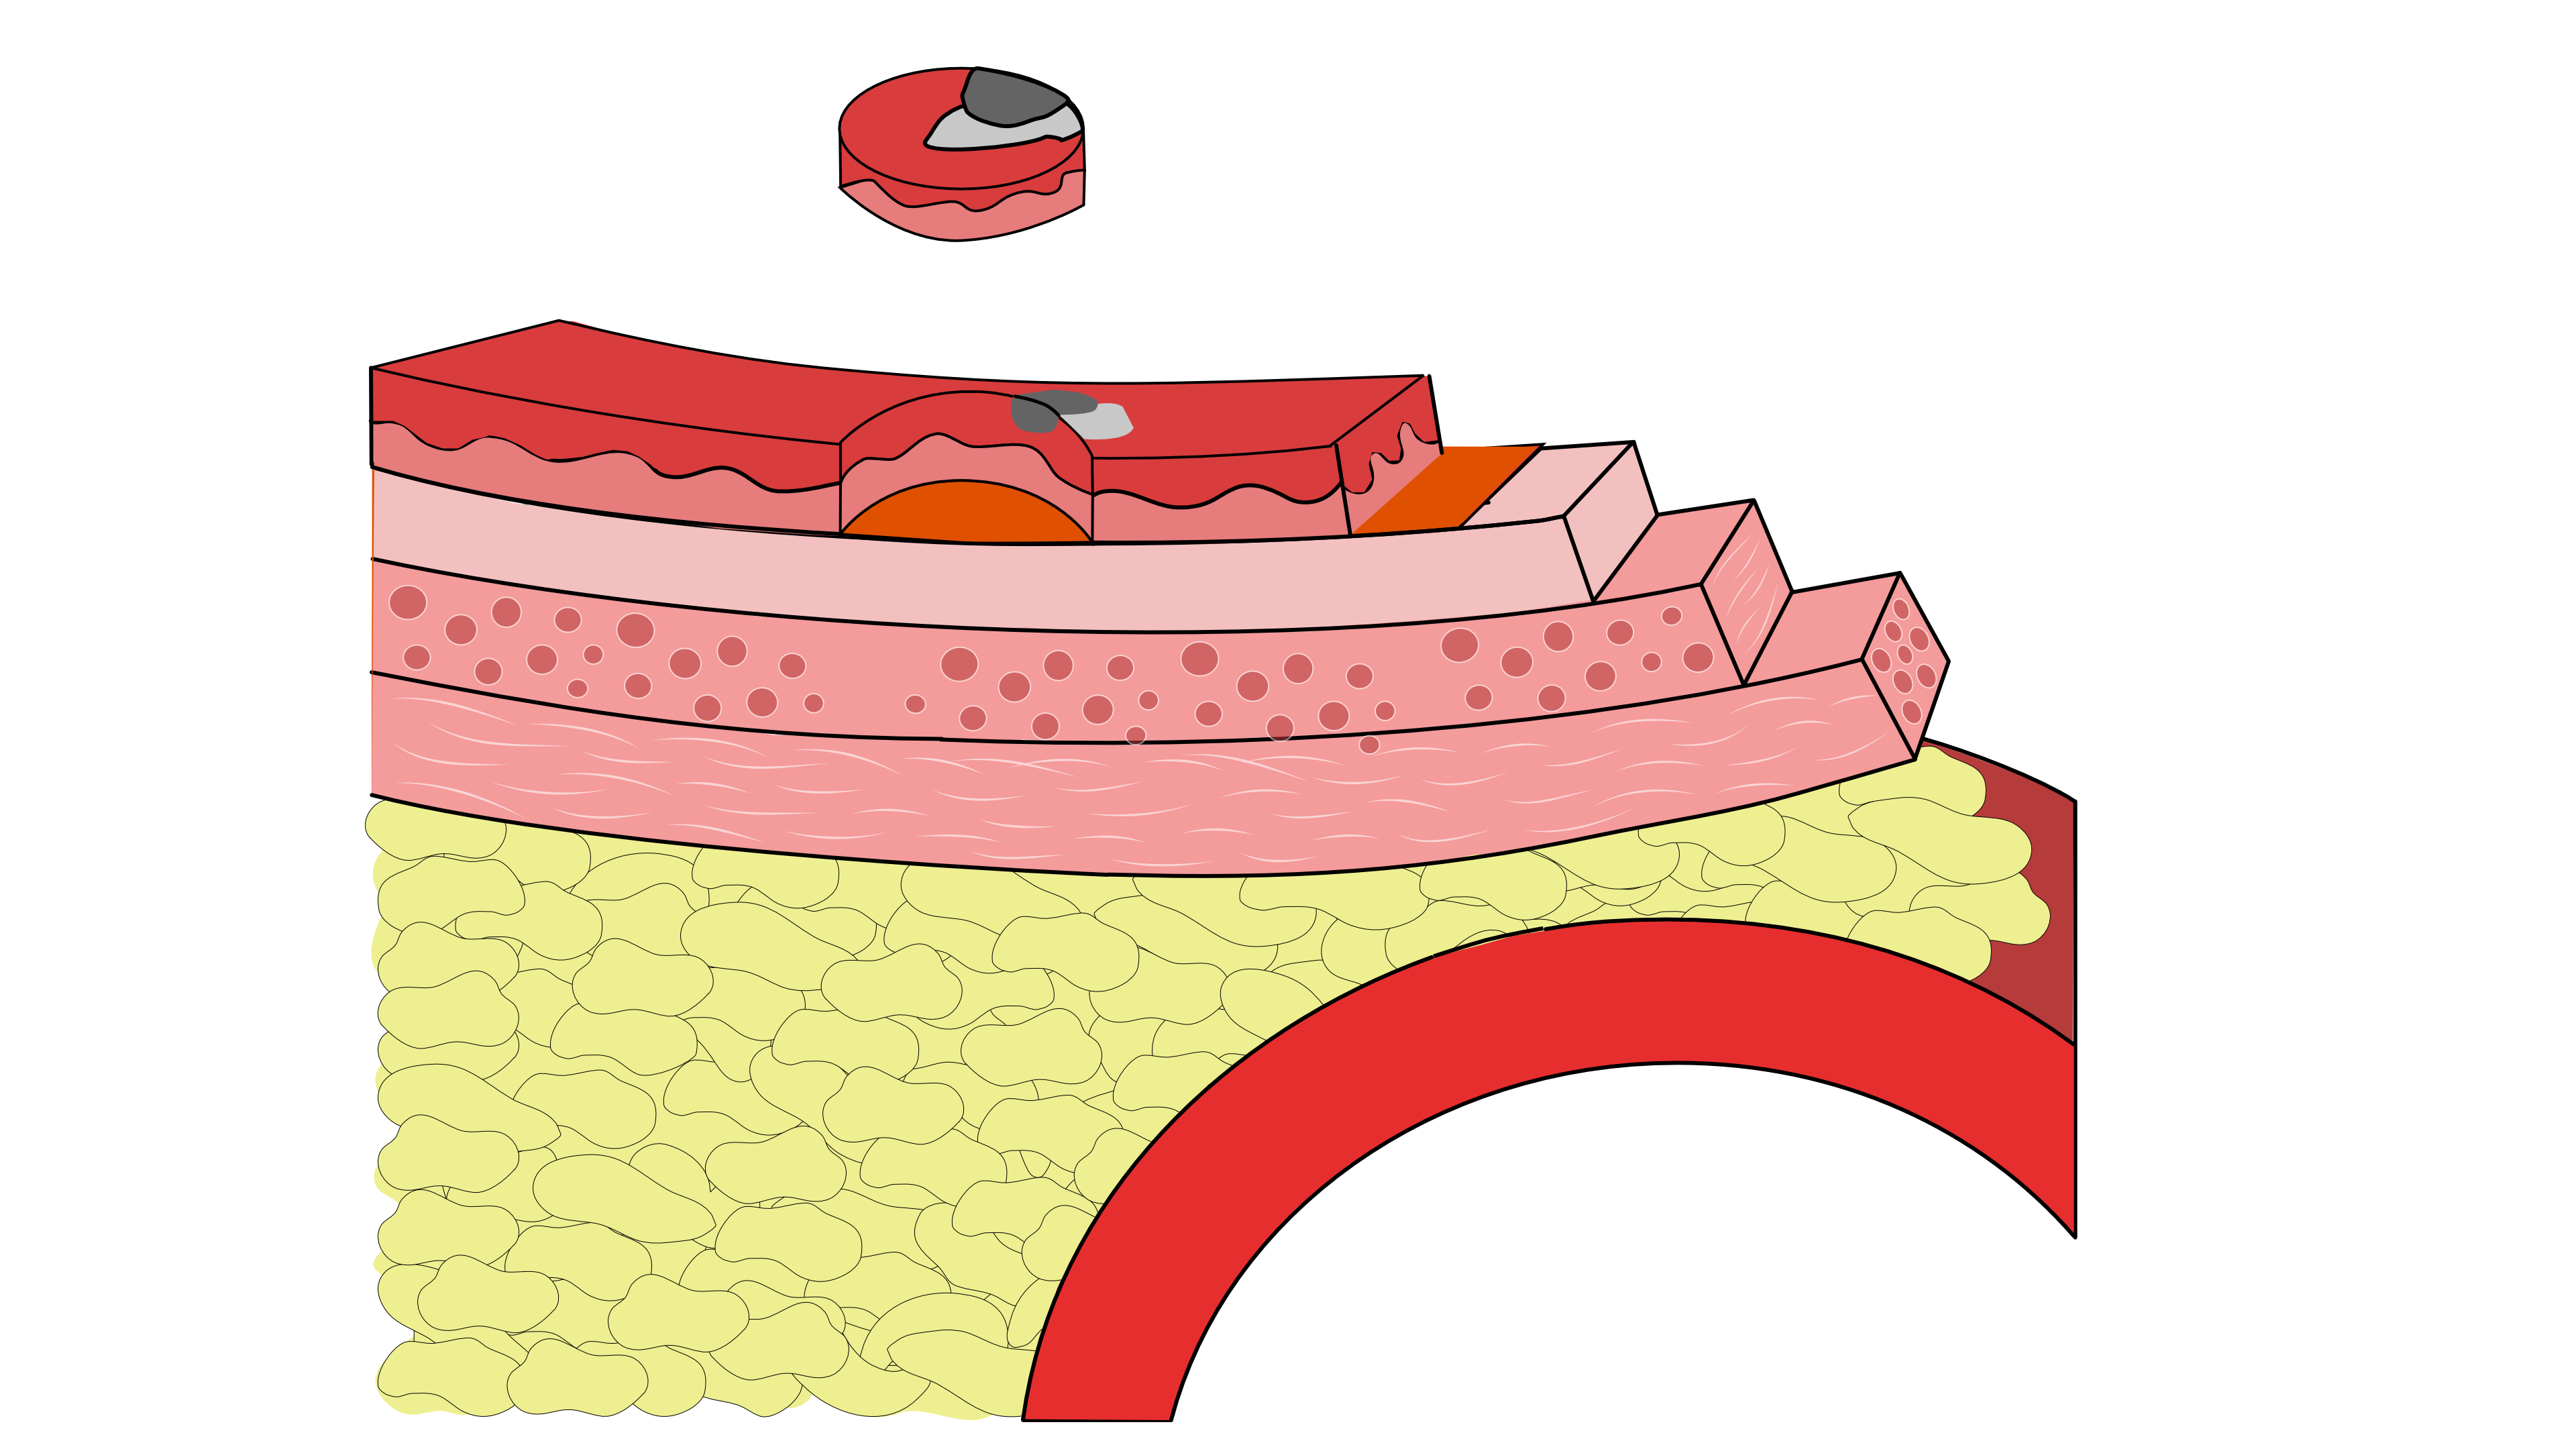
\includegraphics{christmas2004_files/mediabag/emr_unfavorable.png}

\subsection{Endoscopic Mucosal Resection -
Unfavorable}\label{endoscopic-mucosal-resection---unfavorable-1}

\begin{itemize}
\tightlist
\item
  Tumor at edge margin \emph{OR}
\item
  Tumor at deep margin \emph{OR}
\item
  Tumor appears rapidly-growing under microscope
\end{itemize}

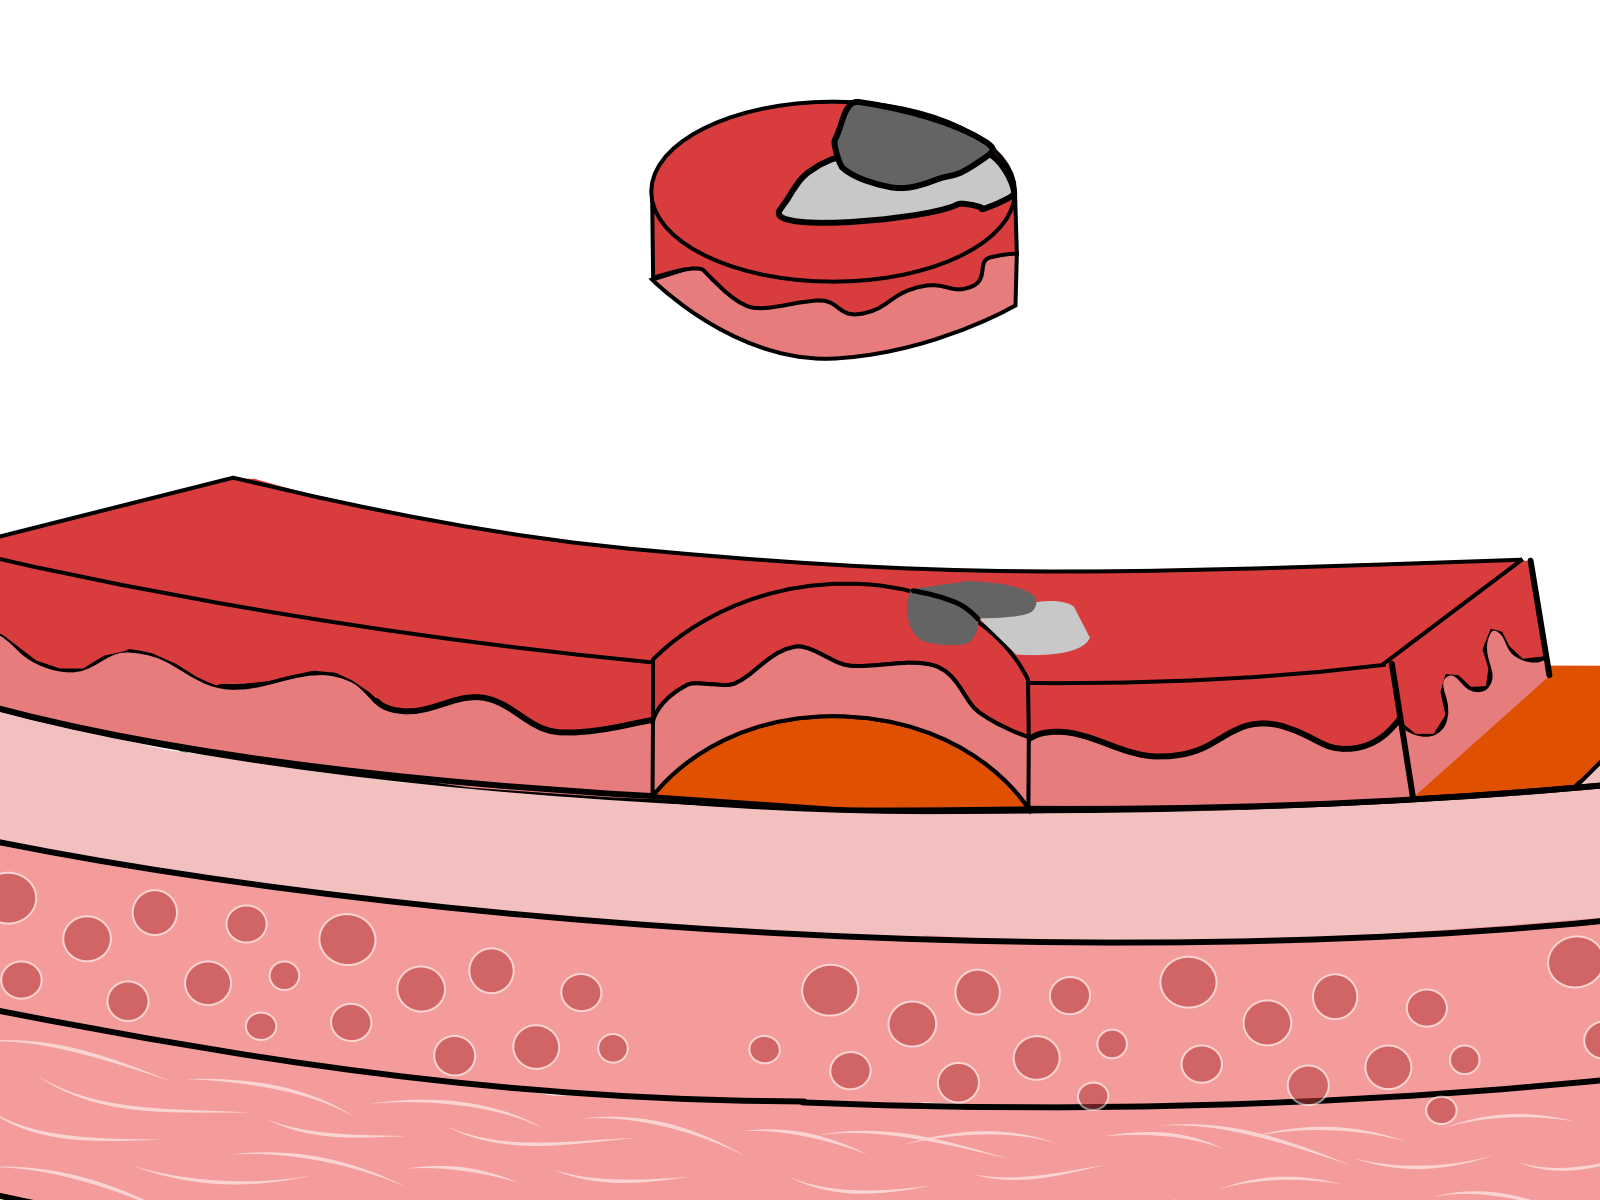
\includegraphics{christmas2004_files/mediabag/emr_unfavorable_1600.png}

Esophagectomy (surgery) is standard recommendation

\subsection{Surgery}\label{surgery}

\href{lci_surgery.htm}{Surgery Slideshow}




\end{document}
